\chapter{Metodologia di ricerca} %\label{1cap:spinta_laterale}
% [titolo ridotto se non ci dovesse stare] {titolo completo}
%

\section{Research question}
L'obiettivo di questo studio empirico consiste nel comprendere se data scientist, software engineer e altre figure sono a conoscenza del problema della software fairness e, nel caso, come trattano quest'ultima dal punto di vista personale e lavorativo. Si raccoglieranno, quindi, pareri da diverse figure lavorative di cui si prevede di riuscire a comprendere, in generale, quanto la fairness sia rilevante durante la progettazione di un sistema che faccia uso di tecniche di machine learning, che tecniche vengono utilizzate per garantirne il rispetto e come gli intervistati si approcciano al problema. In particolare, lo studio cerca di rispondere alla seguente research question: \emph{quali sono le best e bad practice che potrebbero influenzare i livelli di software fairness nello sviluppo di una soluzione fair critical?}\\
Il quesito verrà risposto analizzando i dati ottenuti tramite la somministrazione di un particolare survey, incentrandosi principalmente sulle domande inerenti le practice.

\section{Survey}
\subsection{Design e struttura}
Per rispondere alle research question si è condotto uno studio basato su un survey.\\
Quest'ultimo è formato da 5 sezioni principali, composte da un totale di 26 domande. Tra le domande del survey ne è presente una discriminante utile a comprendere se l'intervistato è adatto o meno alla compilazione; sono presenti due attention check per comprendere se l'intervistato sta compilando le domande con attenzione, quindi senza trascurare le domande e le risposte assegnate. La domanda discriminatoria redigerà l'intervistato alla sezione \emph{conclusione} del survey, a differenza degli attention check. Per questi ultimi, sarà possibile dedurre che l'intervistato abbia effettivamente compilando il survey dando risposte casuali o meno. La risposta scorretta a questa tipologia di domanda non redigerà l'intervistato alla conclusione del survey, bensì verrà analizzata tramite apposito script con conseguente rimozione delle risposte dell'intervistato dal dataset raccolto, al fine di conservare solamente le risposte date con criterio. Riassumendo, il dataset viene pulito in modo da diventare esente, quanto possibile, da risposte insensate.\\
Il survey è stato realizzato tramite la piattaforma Google Forms, la quale:
\begin{itemize}
    \item rende possibile la compilazione del form da molteplici device e browser;
    \item evita che una stessa persona effettui molteplici compilazioni;
    \item salva le risposte nel caso un intervistato si disconnetta dalla compilazione;
    \item offre una vasta varietà di tipologie di domande;
    \item permette l'export delle risposte fornite in modo da poterle elaborare esternamente tramite particolari programmi e script.
\end{itemize}
Il survey è stato progettato in modo da filtrare i partecipanti che avessero un minimo di esperienza con il rispetto della fairness nei sistemi di machine learning, quindi i partecipanti con nessuna esperienza abbandoneranno presto il survey. Tutti i partecipanti del survey sono volontari, la maggior parte di essi individuati tramite la piattaforma Prolific.\\
Sono state adottate particolari guideline durante la progettazione di quest'ultimo siccome un importante obiettivo da raggiungere consiste nell'evitare che l'intervistato abbandoni o inizi a rispondere fornendo risposte superficiali o fuorvianti: ciò può accadere per via del troppo tempo impiegato per compilare il questionario, un numero di domande eccessivo, lessico di difficile comprensione e uso di frasi ambigue. Pertanto, si è deciso di:
\begin{itemize}
    \item strutturare il survey in modo tale che duri 15 minuti circa;
    \item effettuare domande che richiedano l'opinione personale dell'intervistato in modo da catturare la sua attenzione e suscitare interesse;
    \item svolgere una presentazione del survey specificando obiettivi e politiche di privacy, in modo da creare un particolare legame di fiducia con l'intervistato;
    \item ricompensare gli intervistati per la compilazione tramite la piattaforma Prolific;
    \item implementare un processo di follow-up, per avere maggiori informazioni dall'intervistato nel caso quest'ultimo sia interessato a collaborare con lo studio.
\end{itemize}
Si è prestata molta attenzione all'aspetto \emph{privacy} siccome si è ritenuto utile creare un legame di confidenza con l'intervistato, altro aspetto che potrebbe influenzare il modo in cui quest'ultimo risponde alle domande. In particolare, è stato specificato che:
\begin{itemize}
    \item le risposte sono anonime, quindi non si conoscerà la persona a cui faranno riferimento particolari informazioni sensibili;
    \item le risposte saranno sottoposte ad una particolare analisi, la quale verrà poi pubblicata;
    \item le risposte verranno utilizzate solo per fini di ricerca.
\end{itemize}
Le decisioni intraprese circa il design del survey fanno riferimento alle guideline definite da Andrews et al. \cite{andrews2007conducting} utili a creare un particolare livello di fiducia con l'intervistato e a ridurre la probabilità che abbandoni lo studio.

\subsection{Sezioni e domande}

Seguono le sezioni presenti nel survey, di cui per ognuna viene fornita una breve descrizione e l'elenco delle domande che la compongono.\\
Le informazioni fornite circa le sezioni e le domande elencate sono presentate secondo le modifiche svolte a seguito dello studio pilota.

\subsubsection{Introduzione al survey}

Il survey accoglie l'intervistato con un piccolo disclaimer introduttivo, il quale informa l'intervistato circa alcuni aspetti come il tempo in media richiesto per la compilazione, il fatto che la partecipazione sia volontaria e che quando vorrà, l'intervistato, potrà abbandonare la compilazione in qualsiasi momento. Sono presenti informazioni riguardanti anche la raccolta dati, le quali rassicurano l'intervistato circa il fatto che le risposte siano anonime, che saranno utilizzate per svolgere determinate analisi al fine di dedurre nuove informazioni che potranno essere utili per eventuali studi futuri.\\
Il disclaimer si conclude ringraziando in anticipo l'intervistato e avvertendolo del fatto che procedendo alla compilazione avrà dato consenso alle condizioni circa il trattamento dei dati.

\subsubsection{Informazioni sull'utente}

La prima sezione di domande del survey riguarda le informazioni sensibili dell'intervistato: gli vengono chiesti età, gender e provenienza per comprendere se, in qualche modo, la concezione di fairness possa dipendere da tali fattori; viene chiesto il livello di istruzione, la posizione e il ruolo lavorativo, anni di esperienza nel proprio lavoro e nei sistemi di machine learning (domanda discriminatoria) per comprendere se l'intervistato è adatto o meno alla compilazione. È stata prestata particolare attenzione per il genere, attributo decisamente sensibile, al quale si è preferito dare l'opportunità di scegliere più di una risposta nel caso una persona si rispecchi in più generi e una risposta aperta per lasciare la possibilità di specificare un eventuale genere di cui non si è tenuto conto \cite{genderform}. Le domande inerenti ai dati sensibili dell'intervistato sono rese facoltative, quindi può avvalersi della facoltà di non rispondere.

\begin{longtable}{| p{.50\textwidth} | p{.25\textwidth} | p{.15\textwidth} |} 
\hline\textbf{\textit{Domanda}} & \textbf{\textit{Tipo di Domanda}} & \textbf{\textit{Obbligatoria}}\\
\hline
\endhead 

\hline 
Inserisci il tuo codice Prolific

& Risposta breve

& No 

\\ \hline
\rowcolor{Gray!30}
Quanti anni hai?        

&  Scelta multipla

& No

\\ \hline

In quale gender ti rispecchi maggiormente?

& Caselle di controllo

& No

\\ \hline
\rowcolor{Gray!30}
Da dove vieni?        

&  Scelta multipla

& No

\\ 
\hline

Qual è il maggior livello di istruzione che hai conseguito?

& Scelta multipla

& Sì

\\ \hline

\rowcolor{Gray!30}
Qual è la tua posizione lavorativa attuale?        

&  Caselle di controllo

& Sì

\\ \hline

In che settori lavori attualmente?        

&  Caselle di controllo

& Sì

\\ \hline

\rowcolor{Gray!30}
Qual è il tuo ruolo professionale?        

&  Caselle di controllo

& Sì

\\ \hline

Quanti anni di esperienza hai nel ruolo assunto attualmente?        
&  Scelta multipla

& Sì

\\ \hline
\rowcolor{Gray!30}
Hai mai lavorato allo sviluppo di soluzioni AI-Intensive o a sistemi che includono moduli di machine learning?        

&  Scelta multipla

& Sì

\\ \hline
\caption{Domande della sezione \emph{informazioni sull'utente}} % needs to go inside longtable environment
\label{tab:myfirstlongtable}
\end{longtable}

\subsubsection{Come viene approcciata a lavoro la fairness?}

In questa sezione viene fornita una definizione formale di fairness alla quale il survey farà riferimento nelle successive domande. Tale definizione è stata fornita per dare un'idea comune di fairness, utile nel caso in cui qualche intervistato avesse un'idea diversa o comunque ambigua. Le domande di tale sezione cercano di comprendere se e come l'azienda tratta la fairness, esplorando determinati aspetti lavorativi e cercando di comprendere il punto di vista aziendale riguardo tale argomento. È particolarmente interessante, ad esempio, la domanda inerente al livello di maturità dell'azienda circa il rispetto della fairness, quindi la classificazione del modo in cui l'azienda affronta tale problematica. Tale domanda risulta essere un riadattamento del Capability Maturity Model, modello capace di descrivere l'organizzazione aziendale circa lo sviluppo del software \cite{cmm}: in tal caso, la domanda specializza il modello sul trattamento della fairness.  È presente, inoltre, un attention check che chiede all'intervistato quali siano i drink che preferisce bere durante il sabato sera: tra le risposte sono presenti alcune opzioni che non siano drink, cioè \emph{casa} e \emph{calzini}.

\begin{longtable}{| p{.50\textwidth} | p{.25\textwidth} | p{.15\textwidth} |} 
\hline\textbf{\textit{Domanda}} & \textbf{\textit{Tipo di Domanda}} & \textbf{\textit{Obbligatoria}}\\
\hline
\endhead 

\hline 
Secondo la tua opinione, i seguenti aspetti quanto rappresentano la soprastante generica definizione di fairness?

& Griglia a scelta multipla

& Sì 

\\ \hline
\rowcolor{Gray!30}
Considerando le tue esperienze lavorative, quanto vengono applicati i seguenti approcci?

& Griglia a scelta multipla

& Sì 

\\ \hline

Utilizzi altri approcci inerenti al rispetto della fairness?   

&  Risposta breve

& No

\\ \hline
\rowcolor{Gray!30}
Quali drink preferisci durante il sabato sera?

&  Caselle di controllo

& Sì

\\ \hline 
Dati i seguenti ruoli, quali hanno un particolare impatto sulle decisioni inerenti al rispetto della fairness?

& Griglia a scelta multipla

& Sì 

\\ \hline
\rowcolor{Gray!30}
In che livello di maturità rispecchi la tua azienda riguardo il rispetto della fairness?

& Griglia a scelta multipla

& Sì 

\\ \hline
Considerando i seguenti aspetti, se comparati con la fairness quanto pensi possano essere importanti?

& Griglia a scelta multipla

& Sì 

\\ \hline
\caption{Domande della sezione \emph{come viene approcciata a lavoro la fairness?}} % needs to go inside longtable environment
\label{tab:myfirstlongtable}
\end{longtable}

\subsubsection{La fairness durante lo sviluppo della pipeline}

In questa sezione vengono poste due domande utili a comprendere se durante la costruzione delle pipeline si tiene conto dell'aspetto fairness e se vengono utilizzati particolari tool che ne assicurino il rispetto. All'intervistato viene mostrata una generica pipeline di machine learning in modo da fargli comprendere a cosa fa riferimento la domanda nel dettaglio. Anche in questa sezione è presente un attention check, il quale chiede all'intervistato quale numero viene dopo il 3 contando all'indietro.

\begin{longtable}{| p{.50\textwidth} | p{.25\textwidth} | p{.15\textwidth} |} 
\hline\textbf{\textit{Domanda}} & \textbf{\textit{Tipo di Domanda}} & \textbf{\textit{Obbligatoria}}\\
\hline
\endhead 

\hline 
Considerando una generica pipeline di machine learning (come la seguente mostrata tramite immagine), quanto tieni in considerazione l'aspetto fairness durante le seguenti fasi a lavoro?

& Griglia a scelta multipla

& Sì 

\\ \hline
\rowcolor{Gray!30}

Quali tool utilizzi (se ne fai uso) per rispettare la fairness durante la costruzione delle pipeline?

&  Caselle di controllo

& No

\\ \hline

Contando all'indietro dal 5, quale numero segue il 3?

&  Scelta multipla

& Sì

\\ \hline 
\caption{Domande della sezione \emph{la fairness durante lo sviluppo della pipeline}} % needs to go inside longtable environment
\label{tab:myfirstlongtable}
\end{longtable}

\subsubsection{Trattare la fairness}

In questa sezione si chiedono all'intervistato pareri circa quelle che potrebbero essere le cause delle discriminazioni svolte dal sistema e quelle che potrebbero essere le bad e le best practice. Lo scopo è venire a conoscenza sia di pratiche che possano garantire il rispetto della fairness e mitigare eventuali discriminazioni svolte dal sistema e sia pratiche da non seguire siccome potrebbero portare a problemi che non garantiscano il rispetto della fairness. In generale, all'intervistato vengono poste una serie di pratiche che hanno a che fare con il dataset e con il modello predittivo: sarà quest'ultimo a valutare se tali pratiche possano essere considerate come best o bad practice in relazione al rispetto della fairness. Molte delle practice proposte provengono dalla letteratura inerente al machine learning, mentre altre sono ipotizzate e proposte dagli autori del survey.\\
Vengono, inoltre, posti due quesiti aperti in cui si chiedono maggiori informazioni sulle bad e le best practice utilizzate dagli intervistati: purtroppo, nello stato attuale, la ricerca non ha definito alcuna best practice, quindi sarebbe più che utile sapere se molteplici intervistati sono a conoscenza di best e bad practice che, magari, non sono state prese in considerazione nella composizione delle domande.

\begin{longtable}{| p{.50\textwidth} | p{.25\textwidth} | p{.15\textwidth} |} 
\hline\textbf{\textit{Domanda}} & \textbf{\textit{Tipo di Domanda}} & \textbf{\textit{Obbligatoria}}\\
\hline
\endhead 

\hline 
Secondo la tua opinione, quali sono gli attributi sensibili che potrebbero causare discriminazioni?

& Griglia a scelta multipla

& Sì 

\\ \hline
\rowcolor{Gray!30}
Secondo la tua opinione, possono esserci altri attributi sensibili che potrebbero causare discriminazioni? Se sì, quali?

& Risposta breve

& No

\\ \hline
Secondo la tua opinione, quali sono gli aspetti che potrebbero causare discriminazioni?

& Griglia a scelta multipla

& Sì 

\\ \hline
\rowcolor{Gray!30}
Considerando la tua esperienza lavorativa, puoi classificare i seguenti aspetti come bad o best practice?

& Griglia a scelta multipla

& Sì 

\\ \hline
Considerando la tua esperienza lavorativa, ci sono altre bad practice da non adottare?

&  Risposta breve

& No

\\ \hline
\rowcolor{Gray!30}
Considerando la tua esperienza lavorativa, ci sono altre best practice da adottare?

& Risposta breve

& No

\\ \hline
\caption{Domande della sezione \emph{trattare la fairness}} % needs to go inside longtable environment
\label{tab:myfirstlongtable}
\end{longtable}

\subsubsection{Conclusione}

Ultima sezione del survey è quella conclusiva, nella quale si ringrazia l'intervistato per il tempo speso e si chiede la cortesia di lasciare i propri contatti nel caso voglia collaborare con eventuali altre domande di approfondimento. È data possibilità tramite un'apposita domanda di aggiungere nuove informazioni e nuovi dettagli che, magari, non sono stati trattati o che sono stati tralasciati durante il survey.\\
Tale sezione può essere raggiunta compilando correttamente il survey o rispondendo, alla domanda discriminatoria, che non si ha mai lavorato su sistemi di machine learning o che includano un modulo intelligente.

\begin{longtable}{| p{.50\textwidth} | p{.25\textwidth} | p{.15\textwidth} |} 
\hline\textbf{\textit{Domanda}} & \textbf{\textit{Tipo di Domanda}} & \textbf{\textit{Obbligatoria}}\\
\hline
\endhead 

\hline 
Se vuoi, puoi raccontarci di più circa la fairness. Qualsiasi informazione che non abbiamo considerato è importante.

& Paragrafo

& No

\\ \hline
\rowcolor{Gray!30}
Se vuoi rimanere aggiornato riguardo i risultati dello studio o essere contattato per partecipare ad una successiva intervista, scrivi qui il tuo indirizzo email.

& Risposta breve

& No

\\ \hline
\caption{Domande della sezione \emph{conclusione}} % needs to go inside longtable environment
\label{tab:myfirstlongtable}
\end{longtable}

\subsection{Validazione}

Un aspetto cruciale del survey consiste nell'assicurare un particolare livello di qualità, difatti le domande e le risposte sono state più volte revisionate e riformulate al fine di renderle scorrevoli e immediate, con un lessico decisamente semplice e comprensibile da quante più persone possibili. È stato rivisto più volte il numero di domande, cercando di escludere quelle meno rilevanti in modo da evitare che il survey possa risultare troppo lungo. Una volta definita una prima versione del survey è stato condotto uno studio pilota, il che consiste nel far compilare il survey da un piccolo gruppo di persone in modo da poter ottenere pareri utili per migliorare quest'ultimo. Lo studio pilota è stato eseguito da diversi studenti del corso di Software Engineering for Artificial Intelligence della magistrale in Software Engineering dell'Università degli Studi di Salerno: alla conclusione della lezione è stata chiesta la cortesia agli studenti di compilare il questionario e di segnalare eventuali problematiche laddove se ne fossero presentate. In realtà, durante lo studio pilota è stata somministrata una copia del reale survey in modo da tenere separate le risposte ottenute durante questa fase rispetto a quelle ottenute tramite intervistati reali.\\
Pertanto, è stato messo a disposizione degli studenti un link che lasciasse la possibilità di riportare problematiche e suggerimenti: da qui, uno studente ha segnalato il fatto che chiedere obbligatoriamente dati sensibili potrebbe dar fastidio. Pertanto, le domande richiedenti tali dati sono state rese non obbligatorie.\\
Inoltre, il survey dello studio pilota comprende una domanda aggiuntiva posta alla fine di quest'ultimo nella quale si chiede allo studente quanto tempo, orientativamente, ha speso nella compilazione. La maggior parte delle risposte hanno segnalato un tempo più alto rispetto a quello valutato, quindi si è deciso di rimuovere una sezione inizialmente presente nello studio pilota. Tale sezione riguardava la definizione della fairness ed era, a sua volta, suddivisa in due parti: una prima parte chiedeva definizioni teoriche di fairness e bias, mentre una seconda parte forniva una definizione formale di fairness alla quale il survey avrebbe fatto riferimento e chiedeva, in relazione a quest'ultima, quanti anni di esperienza possiede l'intervistato. Quest'ultima domanda era discriminatoria ed era utile al punto da filtrare gli intervistati che non hanno esperienza con la definizione di fairness fornita. Si è valutato di rimuovere tale sezione siccome non era ritenuta essenziale ai fini dello studio da svolgere, mentre la definizione formale di fairness fornita è stata spostata nel capitolo \emph{come viene approcciata a lavoro la fairness?}\\
Dopo aver apportato le modifiche elencate, il survey è stato diffuso tramite la piattaforma Prolific e somministrato a 200 partecipanti circa.

\subsection{Reclutamento dei partecipanti}
Uno dei primi quesiti sorti durante la progettazione del survey consisteva nello stabilire quali fossero le tipologie di intervistati al quale sottomettere il survey. Da un'apposita sessione di brainstorming, è stato valutato possa essere idoneo considerare le seguenti figure:
\begin{itemize}
    \item Data Scientist;
    \item Software Engineer;
    \item Data Engineer;
    \item Manager oppure Project Manager;
    \item Software Analyst;
    \item Software Architect.
\end{itemize}
Nulla vieta la somministrazione del survey ad altre figure, difatti nell'apposita domanda che chiede il proprio ruolo professionale nella sezione introduttiva è possibile dichiarare anche ruoli diversi. L'idea sta nel fatto che possa essere una buona idea poter classificare idee e ragionamenti circa il rispetto della fairness a seconda del ruolo professionale, in modo da individuare particolari scuole di pensiero in dipendenza da quest'ultimo.\\
Gli intervistati sono stati individuati principalmente tramite la piattaforma Prolific, la quale permette di reclutare molteplici partecipanti pagando una particolare somma per ognuno di essi. Si è provato ad attrarre un'altra fetta di partecipanti tramite il social network LinkedIn, pubblicando su alcune community inerenti al machine learning un post in cui si chiedeva la compilazione del survey, dando una piccola anticipazione riguardante i contenuti del survey e l'importanza di contribuire a tale studio. Essendo LinkedIn utilizzato da molteplici professionisti si è supposto che la partecipazione al survey da questi ultimi sia pienamente volontaria e svolta con massima serietà, siccome difficilmente un utente non interessato si prenderebbe la briga di compilare un questionario del genere e, nel caso ipotetico accada, ci penserebbero le domande discriminatorie e gli attention check a filtrare le risposte non valide. Come per lo studio pilota, anche per LinkedIn è stata creata una copia del survey non comprendente la domanda in cui si chiede l'identificativo utente di Prolific.\\
Tornando alle figure da considerare adatte alla compilazione del survey, Prolific permette di definire alcuni criteri per i quali è possibile scegliere il pubblico adatto alla somministrazione. Il problema è che i filtri messi a disposizione da Prolific sono abbastanza generici e non permettono di filtrare figure come Data Scientist, Software Engineer, etc.\\
Pertanto, oltre allo stabilire i filtri generici proposti ad Prolific, nella descrizione del survey è stata esplicitamente richiesta la partecipazione di ruoli adeguati all'argomento; altrimenti, si è pregati di non compilare il survey. I filtri impostati tramite Prolific sono i seguenti:
\begin{itemize}
    \item Saper parlare e scrivere in inglese fluente;
    \item Amare il proprio lavoro e saper rispettare i propri colleghi;
    \item Aver avuto esperienze lavorative in campi scientifici;
    \item Aver conseguito almeno il diploma delle scuole superiori;
    \item Essere disposti ad accettare condizioni inerenti al trattamento dei dati;
    \item Saper usare un computer o un cellulare.
\end{itemize}

\section{Minacce alla validità}
La validità di un esperimento permette di valutare se il risultato di quest'ultimo rispecchia effettivamente il fenomeno studiato. Le minacce alla validità sono considerate essere tutte le variabili di disturbo che possano influenzare il risultato dell'esperimento.\\
\subsection{Minacce alla validità interna}
Una delle maggiori sfide quando si parla di compilazione di un questionario riguarda la ricerca dei partecipanti e che questi ultimi siano adatti al dominio trattato. Riguardo il survey trattato, il partecipante ideale dovrebbe possedere conoscenze ed esperienze pregresse circa il machine learning, il tutto accompagnato da un particolare affezionamento ad importanti argomenti sociali, in questo caso l'equità sociale. Come già anticipato, la ricerca dei partecipanti è stata svolta tramite due piattaforme: LinkedIn, social per il lavoro, e Prolific, piattaforma realizzata per la ricerca dei partecipanti.
\begin{itemize}
    \item La ricerca dei partecipanti tramite LinkedIn è stata condotta pubblicando post su appositi gruppi che avessero come topic principale il machine learning. Il post spiega molto velocemente al lettore gli obiettivi della ricerca, dando maggiore rilevanza al perché: ci si è incentrati molto sul tema dell'equità sociale in modo da attrarre partecipanti che tenessero molto alla causa e per fargli comprendere quanto sia importante il loro contributo. Lo scopo del post era, quindi, quello di attrarre i partecipanti suscitando il loro interesse verso la problematica. Il problema è che per tale categoria di partecipanti non era prevista una ricompensa o un qualsiasi tipo di incentivo per la partecipazione se non l'affezione verso la causa; difatti, si è ricevuto un numero irrilevante di risposte le quali si è deciso di scartare, anche perché poco significative;
    \item La piattaforma Prolific permette di scegliere i partecipanti tramite un apposito sistema di filtraggio nel quale vengono impostate particolari caratteristiche che i partecipanti dovranno possedere per poter partecipare. Il problema è che tali filtri sono abbastanza generici, quindi si è scelto di inserire una domanda nel questionario che permettesse di filtrare i partecipanti senza esperienza nei sistemi machine learning. Inoltre, tramite Prolific è stato possibile invogliare i partecipanti consegnando loro una ricompensa, precisamente un compenso economico previsto dalla piattaforma stessa.
\end{itemize}
Nonostante tutto non si è in grado di garantire un campione privo di bias, quindi sono state effettuate operazioni di pulizia sul dataset escludendo partecipanti senza esperienza, chi non ha rispettato gli attention check e altri partecipanti secondo alcune indicazioni della piattaforma elencate nell'apposito paragrafo di pulizia dei dati.\\
\subsection{Minacce alla validità esterna}
Essendo i partecipanti reclutati tramite la piattaforma Prolific, non c'è stato modo di scegliere la loro provenienza. Tra i reclutati, vedremo nell'apposito paragrafo di analisi dei dati, molti di loro provengono dall'Europa e dall'Africa, mentre per dagli altri continenti si hanno pochissimi partecipanti per i quali potrebbe essere sbagliato generalizzare i risultati. Pertanto, sarebbe corretto replicare lo studio concentrandosi sui continenti per i quali si hanno ricevuto poche o nessuna risposta. Si potrebbe valutare di replicare lo studio anche su partecipanti il cui background lavorativo sia diverso rispetto a quelli più diffusi nelle risposte ottenute, dato che molti dei partecipanti assumono i ruoli di Software Engineer, Data Scientist e Manager: sarebbe interessante generalizzare i risultati anche in base al ruolo lavorativo.\\
\subsection{Minacce alla validità di costrutto}
Le minacce alla validità di costrutto fanno riferimento alla relazione tra ipotesi e osservazioni: nel caso specifico del survey, si farà riferimento al design di quest'ultimo. Come già anticipato, il survey è stato realizzato sviluppando domande dal lessico semplice, di semplice comprensione e non ambigue, in modo tale che chiunque potesse comprenderle senza problemi. Sono state definite, inoltre, domande a risposta aperta in modo da lasciare al partecipante la libertà di fornire eventuali informazioni aggiuntive; tali domande sono state rese facoltative in modo da non costringere alcun partecipante a lasciare forzatamente una risposta sulla quale, magari, non avrebbe nulla da dire. Per osservare se il design del survey fosse funzionale e qualitativamente accettabile, è stato svolto uno studio pilota a cui hanno preso parte diversi studenti dell'Università degli Studi di Salerno che avessero conoscenze, anche basilari, circa il machine learning. Ciò ha reso possibile modifiche al survey laddove alcune domande fossero poco comprensibili o ambigue e modifiche in termini di tempo impiegato per la compilazione. Piuttosto, sarebbe considerabile utile replicare la compilazione del sondaggio ad altri partecipanti per ottenere nuove informazioni e nuovi punti di vista di cui si potrebbe non aver tenuto tenuto.\\
\subsection{Minacce alla validità di conclusione}
Le minacce alla validità di conclusione riguardano le metodologie utilizzate per l'analisi dei dati, le quali serviranno anche per formalizzare i risultati. Il dataset di risposte è stato analizzato tramite strumenti di statistica descrittiva, analizzando dati sia di tipologia qualitativa che quantitativa. Riguardo quest'ultima categoria, è necessario svolgere delle trasformazioni di scala per alcune domande di tipologia \emph{a scelta multipla}, laddove ci fosse la necessità di preferire un'analisi quantitativa rispetto alla qualitativa. Inoltre, si è sentita la necessità di dover applicare delle abbreviazioni alle etichette presenti in domande a scelta multipla. Le trasformazioni di scala e la creazione di abbreviazioni sono attività svolte durante la fase di preparazione del dataset, la quale precede la fase dell'analisi dei dati. Infine, sono stati adeguatamente valutate le metodologie di rappresentazione e descrizione dei dati, utilizzando appositi grafici di semplice comprensione.

\chapter{Analisi dei dati e risultati di ricerca}
\section{Preparazione del dataset}
\subsection{Pulizia dei dati}
Il survey è stato compilato da circa 200 persone in poche ore, di cui circa 130 hanno passato la domanda discriminatoria inerente all'esperienza pregressa sui sistemi di machine learning. In ogni caso, tali partecipanti vanno ricompensati tramite Prolific, il quale lascia all'organizzatore del survey la possibilità di permettere il pagamento della quota ad un partecipante o di rifiutarlo: in quest'ultimo caso bisogna avere buoni motivi per negare il pagamento al partecipante. Un ottimo motivo è la risposta errata ad almeno un attention check, la quale dimostra che l'utente sta rispondendo senza prestare attenzione.\\
Le risposte date negli attention check sono state analizzate manualmente una ad una per ben due volte, al fine di essere sicuri circa chi escludere dal pagamento. Sono stati rilevati ben 17 partecipanti che hanno risposto erroneamente ad almeno un attention check. Sono stati, inoltre, esclusi automaticamente da Prolific alcuni partecipanti che hanno deciso di abbandonare prematuramente lo studio e alcuni che non hanno fornito il completation code, il quale serve a dimostrare che il questionario è stato effettivamente compilato.\\
In primo momento, quindi, sono state rimosse dal dataset tutte le risposte date dai soggetti contrassegnati come rifiutati per il pagamento. Successivamente, si è proceduto con la rimozione delle risposte da parte dei soggetti che hanno ammesso di non avere alcuna esperienza con i sistemi di machine learning, quindi tutti i soggetti che non hanno passato la domanda discriminatoria e che hanno concluso anticipatamente la compilazione del survey. I partecipanti che verranno, quindi, effettivamente considerati durante lo studio sono 115.\\
Riguardo il survey pubblicato sul LinkedIn, sono state ricevute solamente due risposte ritenute poco utili ai fini dell'analisi siccome ricevute da figure professionali per nulla attinenti al machine learning e alla fairness. Per tale motivo, si è deciso di considerare solamente le risposte ricevute tramite la piattaforma Prolific.
\subsection{Partizione del dataset e research question}
Siccome il questionario comprende anche una serie di domande legate ad altri quesiti di ricerca esplorabili, ai fini dell'analisi utile a rispondere alla research question considerata per questo studio si andrà a lavorare su una partizione del dataset complessivo. Precisamente, verranno escluse dall'analisi le domande poste nelle rispettive sezioni \emph{come viene approcciata a lavoro la fairness?} e \emph{La fairness durante lo sviluppo della pipeline}.\\
La partizione interessata sarà composta dalle domande delle seguenti sezioni:
\begin{itemize}
    \item\emph{Informazioni sull'utente}, per l'analisi dei dati demografici come sesso, provenienza, età e per comprendere quanto sia generalizzabile il dataset;
    \item\emph{Trattare la fairness}, per l'analisi circa quali potrebbero essere le cause scatenanti le discriminazioni e quali potrebbero essere le best e bad practice introducibili in letteratura.
\end{itemize}
Piuttosto, sarà data maggiore rilevanza dalla sezione \emph{Trattare la fairness} dato che, per rispondere alla research question, sarà necessario individuare le cause delle discriminazioni ed eventuali best practice per mitigarle quanto possibile.
\subsection{Trasformazioni di scala e abbreviazioni}
Il survey è composto da particolari domande che permettono di fornire risposte qualitative. Pertanto, ai fini delle analisi statistiche, alcune di queste domande subiranno trasformazioni di scala in modo da poter manipolare i risultati in maniera più semplice. Difatti, seguono le domande le cui risposte hanno subito trasformazioni di scala:
\begin{itemize}
    \item Secondo la tua opinione, quali sono gli attributi sensibili che potrebbero causare discriminazioni?\\
    \begin{longtable}{| p{.25\textwidth} | p{.35\textwidth} |}
      \hline\textbf{\textit{Scala quantitativa}} & \textbf{\textit{Valore qualitativo}}
        \\ \hline
        \rowcolor{Gray!30}
        1 & Sicuramente no
        \\ \hline
        2 & Probabilmente no
        \\ \hline
        \rowcolor{Gray!30}
        3 & Neutro
         \\ \hline
        4 & Probabilmente sì
        \\ \hline
        \rowcolor{Gray!30}
        5 & Sicuramente sì
        \\ \hline
        \caption{Scale per la domanda circa le cause delle discriminazioni} % needs to go inside longtable environment
        \label{tab:myfirstlongtable}
    \end{longtable}
    \item Secondo la tua opinione, quali sono gli aspetti che potrebbero causare discriminazioni?\\
    \begin{longtable}{| p{.25\textwidth} | p{.35\textwidth} |}
      \hline\textbf{\textit{Scala quantitativa}} & \textbf{\textit{Valore qualitativo}}
        \\ \hline
        \rowcolor{Gray!30}
        1 & Sicuramente no
        \\ \hline
        2 & Probabilmente no
        \\ \hline
        \rowcolor{Gray!30}
        3 & Neutro
         \\ \hline
        4 & Probabilmente sì
        \\ \hline
        \rowcolor{Gray!30}
        5 & Sicuramente sì
        \\ \hline
        \caption{Scale per la domanda circa le cause delle discriminazioni (2)} % needs to go inside longtable environment
        \label{tab:myfirstlongtable}
    \end{longtable}
    \item Considerando la tua esperienza lavorativa, puoi classificare i seguenti aspetti come bad o best practice?
    \begin{longtable}{| p{.25\textwidth} | p{.35\textwidth} |}
      \hline\textbf{\textit{Scala quantitativa}} & \textbf{\textit{Valore qualitativo}}
        \\ \hline
        \rowcolor{Gray!30}
        1 & Sicuramente è una BAD practice
        \\ \hline
        2 & Molto probabilmente è una BAD practice
        \\ \hline
        \rowcolor{Gray!30}
        3 & Probabilmente è una BAD practice
         \\ \hline
        4 & C'è la possibilità sia una BAD practice
        \\ \hline
        \rowcolor{Gray!30}
        5 & Occasionalmente potrebbe essere una BAD practice
        \\ \hline
        6 & Neutro
        \\ \hline
        \rowcolor{Gray!30}
        7 & Occasionalmente potrebbe essere una BEST practice
         \\ \hline
        8 & C'è la possibilità sia una BEST practice
        \\ \hline
        \rowcolor{Gray!30}
        9 & Probabilmente è una BEST practice
        \\ \hline
        10 & Molto probabilmente è una BEST practice
        \\ \hline
        \rowcolor{Gray!30}
        11 & Sicuramente è una BEST practice
         \\ \hline
        \caption{Scale per la domanda circa la classificazione in best e bad practice} % needs to go inside longtable environment
        \label{tab:myfirstlongtable}
    \end{longtable}
\end{itemize}

In quest'ultima domanda in particolare è mostrato un elenco di practice al fine di comprendere, secondo l'opinione dei partecipanti, se possano essere classificabili come best oppure bad. Al fine di semplificare l'etichettatura dei grafici posti nel paragrafo inerente all'analisi dei dati, tali practice verranno illustrate tramite un particolare identificativo.

\begin{itemize}
    \item Considerando la tua esperienza lavorativa, puoi classificare i seguenti aspetti come bad o best practice?
    \begin{longtable}{| p{.25\textwidth} | p{.35\textwidth} |}
      \hline\textbf{\textit{Identificatore}} & \textbf{\textit{Practice proposta}}
        \\ \hline
        \rowcolor{Gray!30}
        P1 & Svolgimento di attività di data balancing basate sulle feature sensibili
        \\ \hline
        P2 & Esecuzione del processo di training del modello principalmente sulle feature sensibili
        \\ \hline
        \rowcolor{Gray!30}
        P3 & Svolgimento di interview e focus groups al fine di elicitare requisiti inerenti la fairness
         \\ \hline
        P4 & Utilizzo di combinazioni di modelli (ensemble learning)
        \\ \hline
        \rowcolor{Gray!30}
        P5 & Tuning degli hyperparameter
        \\ \hline
        P6 & Selezione di uno specifico algoritmo di machine learning per il rispetto delle assunzioni legate alla fairness
        \\ \hline
        \rowcolor{Gray!30}
        P7 & Svolgimento di attività di validazione e testing su un dataset perfettamente bilanciato
         \\ \hline
        P8 & Considerare la fairness un aspetto prioritario durante la fase di analisi dei requisiti
        \\ \hline
        \rowcolor{Gray!30}
        P9 & Risoluzione di overfitting e underfitting tramite un particolare assegnamento ai pesi
        \\ \hline
        P10 & Particolare assegnamento ai pesi in modo da rendere il modello più preciso nelle predizioni
        \\ \hline
        \rowcolor{Gray!30}
        P11 & Rimozione delle feature sensibili dal dataset
         \\ \hline
        P12 & Confronto di un modello che fa uso di attributi sensibili con un modello che non ne fa uso
        \\ \hline
        \rowcolor{Gray!30}
        P13 & Esecuzione del processo di training su un dataset perfettamente bilanciato
         \\ \hline
        P14 & Svolgimento di attività di validazione su una partizione contenente solo soggetti discriminati
        \\ \hline
        \rowcolor{Gray!30}
        P15 & Aggiunta di nuovi record nel dataset al fine di avvantaggiare gli individui discriminati
        \\ \hline
        P16 & Svolgimento di manutenzione ed evoluzione considerando i cambiamenti dei dati nel tempo
        \\ \hline
        \rowcolor{Gray!30}
        P17 & Assegnazione di valori casuali ai pesi del modello
         \\ \hline
        \caption{Identificatori delle practice proposte nel survey} % needs to go inside longtable environment
        \label{table-root-id-2}
    \end{longtable}
\end{itemize}

Ragionamento analogo viene applicato per la domanda circa gli aspetti inerenti al machine learning che potrebbero causare discriminazioni:

\begin{itemize}
    \item Secondo la tua opinione, quali sono gli aspetti che potrebbero causare discriminazioni?
    \begin{longtable}{| p{.25\textwidth} | p{.35\textwidth} |}
      \hline\textbf{\textit{Identificatore}} & \textbf{\textit{Aspetto}}
        \\ \hline
        \rowcolor{Gray!30}
        MLA1 & Dimensione del dataset
        \\ \hline
        MLA2 & Qualità dei dati nel dataset
        \\ \hline
        \rowcolor{Gray!30}
        MLA3 & Bilanciamento del dataset
         \\ \hline
        MLA4 & Numero di feature
        \\ \hline
        \rowcolor{Gray!30}
        MLA5 & Feature sensibili
        \\ \hline
        MLA6 & Feature ridondanti
        \\ \hline
        \rowcolor{Gray!30}
        MLA7 & Funzione ipotesi del modello
         \\ \hline
        MLA8 & Algoritmo di machine learning
        \\ \hline
        \rowcolor{Gray!30}
        MLA9 & Assegnazione degli hyperparameter
        \\ \hline
        MLA10 & Tempo impiegato per il training
        \\ \hline
        \rowcolor{Gray!30}
        MLA11 & Fase di verifica e/o validazione
         \\ \hline
        MLA12 & Considerazioni circa l'evoluzione dei dati e dell'ambiente
        \\ \hline
        \rowcolor{Gray!30}
        MLA13 & Svolgimento di attività di validazione su una partizione contenente solo soggetti discriminati
         \\ \hline
        \caption{Identificatori degli aspetti causa di discriminazioni} % needs to go inside longtable environment
        \label{table-root-id-1}
    \end{longtable}
\end{itemize}


\section{Analisi dei dati}
Prima di discutere i dati utili a rispondere alla research question, è interessante conoscere il campione di partecipanti che ha contribuito allo studio. Precisamente, verranno analizzate i dati demografici da loro riportati per comprendere quanto sia generalizzabile il campione. Dopodiché, verranno analizzati i dati inerenti a quelle che potrebbero essere le cause delle discriminazioni svolte dai sistemi intelligenti e quelli che potrebbero essere le practice da adottare o di cui fare a meno quando si lavora su sistemi machine learning.

\subsection{Conoscere i partecipanti}
Come anticipato durante il paragrafo inerente alla pulizia dei dati, i partecipanti che hanno compilato il survey erano circa 200, ma per l'analisi dei dati ne verranno considerati solamente 115 siccome molti di essi sono stati filtrati per via di esperienza pregressa non idonea allo studio, abbandono e risposte non sensate. Si ribadisce, quindi, che tutti i partecipanti filtrati hanno esperienza pregressa con i sistemi di machine learning.\\

\begin{figure}[h!]
    \centering
    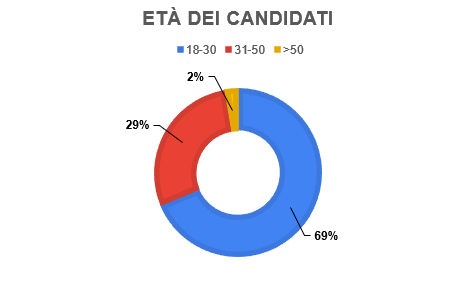
\includegraphics[width=1\textwidth]{figure/data-analysis/eta.png}
    \caption{Distribuzione dei partecipanti in base all'età}
    \label{im-a-part-1}
\end{figure}

Analizzando l'età dei partecipanti (figura \ref{im-a-part-1}) si nota da subito che molti di essi rientrano nella fascia tra i 18 e i 30 anni, precisamente 79 partecipanti (69\%); abbastanza gettonata è anche la fascia tra i 31 e i 50 anni, composta da 33 partecipanti (29\%); infine, sono presenti 3 partecipanti con età che va oltre i 50 anni (2\%). È molto interessante comprendere, quindi, che la maggior parte dei partecipanti che hanno lavorato su sistemi di machine learning siano decisamente giovani, il che è un bene siccome è, oggigiorno, la categoria che ha più a cuore temi sensibili proprio come l'equità di sesso, di razza e così via. Fa piacere sapere che tra i partecipanti siano presenti persone di maggiore età che, non solo si interessano dell'argomento fairness, porteranno sicuramente maggiore maturità professionale.\\

\begin{figure}[h!]
    \centering
    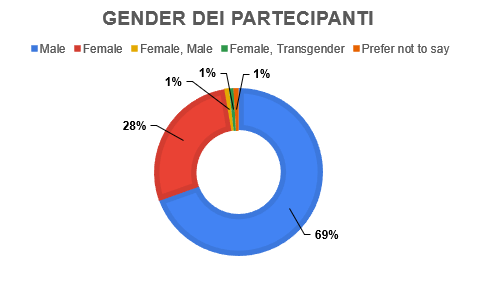
\includegraphics[width=1\textwidth]{figure/data-analysis/gender.png}
    \caption{Distribuzione dei partecipanti in base al gender}
    \label{im-a-part-2}
\end{figure}

È stato analizzato anche il gender dei partecipanti (figura \ref{im-a-part-2}), cioè il sesso in cui si identificano. Tale quesito ha permesso ai partecipanti di selezionare più di una sola risposta siccome si comprende possano esserci persone che si identificano in molteplici sessi. Difatti, sono state ricevute due risposte (2\%) nelle quali i partecipanti si sono rispettivamente identificati come Femmina, Maschio e come Femmina, Transgender. È stata anche data la possibilità di non comunicare il proprio gender ed un partecipante (1\%) ha preferito non esprimersi. Riguardo i restanti, invece, 80 partecipanti (69\%) si identificano come Maschio, mentre altri 32 (28\%) si identificano come Femmina. È stata data quanta più libertà possibile in questa domanda in modo tale che nessuno possa essersi sentito discriminato, limitandosi a scegliere un unico sesso che li rappresenti anziché molteplici.\\

\begin{figure}[h!]
    \centering
    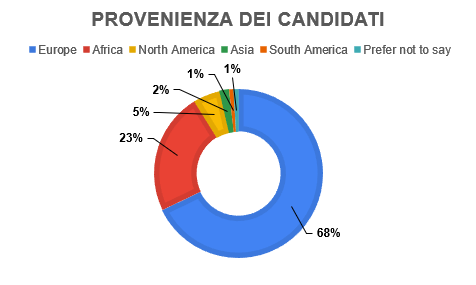
\includegraphics[width=1\textwidth]{figure/data-analysis/prov.png}
    \caption{Distribuzione dei partecipanti in base alla provenienza}
    \label{im-a-part-3}
\end{figure}

Riguardo la provenienza dei partecipanti (figura \ref{im-a-part-3}), il campione è particolarmente concentrato in Europa (68\%), in secondo piano è ben presente anche l'Africa (23\%). Diversi partecipanti provengono anche dal Nord America (5\%), dal Sud America (1\%) e dall'Asia (2\%), ma sono minoranze rispetto ai due continenti inizialmente elencati. Inoltre, un partecipante (1\%) ha preferito non comunicare il proprio continente di provenienza. Da tali dati si comprende il fatto che si possa mettere in discussione la generalizzabilità dei risultati siccome diversi continenti sono molto meno rappresentati: ciò può essere dovuto dal fatto che Prolific è una piattaforma britannica, quindi la minoranza di partecipanti provenienti dall'America e dall'Asia può essere dovuta alla poca o mancata pubblicità della piattaforma in tali continenti.\\

\begin{figure}[h!]
    \centering
    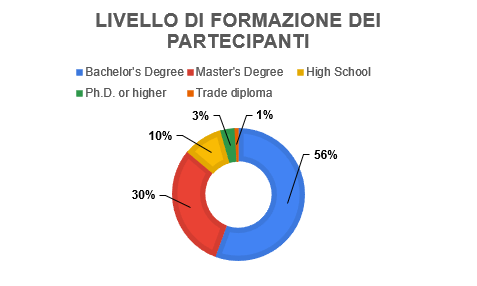
\includegraphics[width=1\textwidth]{figure/data-analysis/formazione.png}
    \caption{Distribuzione dei partecipanti in base alla formazione}
    \label{im-a-part-4}
\end{figure}

\begin{figure}[h!]
    \centering
    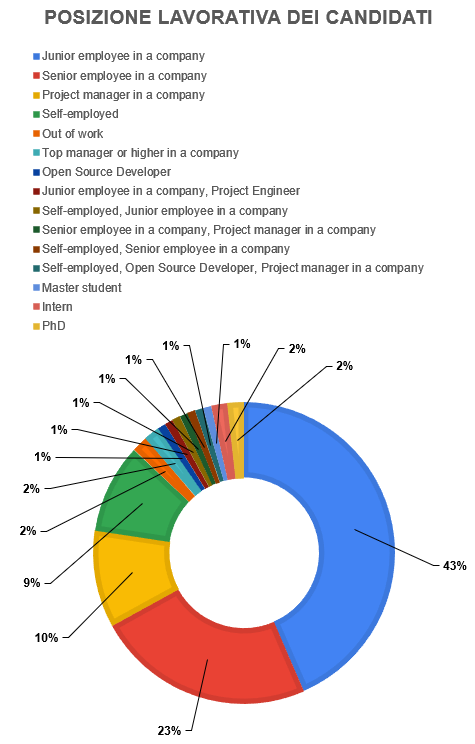
\includegraphics[width=360pt]{figure/data-analysis/lavoro.png}
    \caption{Distribuzione dei partecipanti in base alla posizione lavorativa}
    \label{im-a-part-5}
\end{figure}

\begin{figure}[h!]
    \centering
    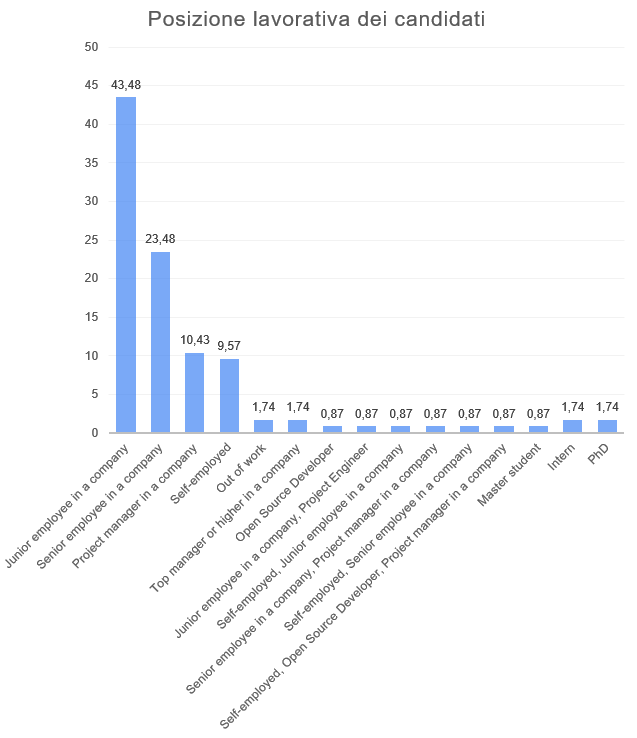
\includegraphics[width=1\textwidth]{figure/data-analysis/lavoro2.png}
    \caption{Frequenze delle posizioni lavorative dei partecipanti}
    \label{im-a-part-6}
\end{figure}

\begin{figure}[h!]
    \centering
    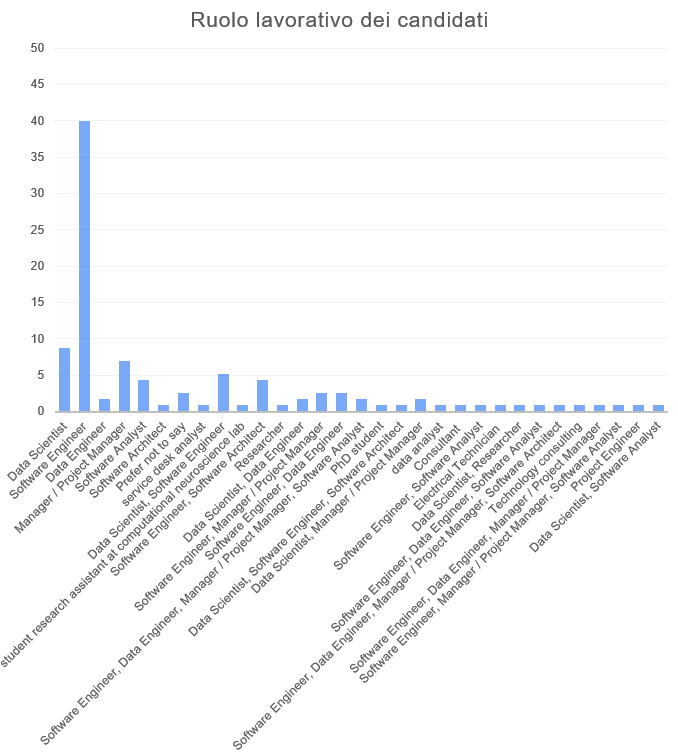
\includegraphics[width=1\textwidth]{figure/data-analysis/ruoli.png}
    \caption{Frequenze dei ruoli lavorativi dei partecipanti}
    \label{im-a-part-7}
\end{figure}

\begin{figure}[h!]
    \centering
    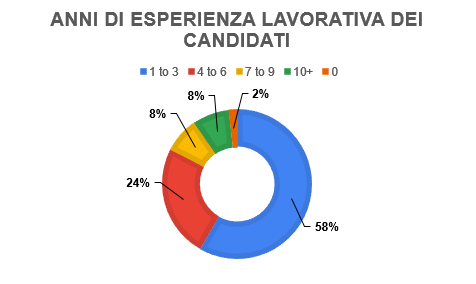
\includegraphics[width=1\textwidth]{figure/data-analysis/anni.png}
    \caption{Distribuzione dei partecipanti in base all'età}
    \label{im-a-part-8}
\end{figure}

Il livello di formazione dei partecipanti (figura \ref{im-a-part-4}) è un indicatore sicuramente molto importante per lo studio siccome è necessario conoscere basi teoriche di machine learning e sviluppo software per rispondere con consapevolezza alle domande del survey. Per semplicità, è stato chiesto ai candidati di fornire il loro titolo di studi più alto ottenuto. Pertanto, si osserva che la stragrande maggioranza dei partecipanti possiede una laurea triennale (89\% complessivo), mentre i restanti (11\% complessivo) possiede un diploma. Precisamente, 64 candidati possiedono solo la laurea triennale (56\%), in 35 possiedono la laurea magistrale (30\%), in 4 possiedono il dottorato o un titolo superiore (3\%), in 11 possiedono un diploma di istruzione superiore (10\%) e una sola persona possiede un diploma professionale (1\%).\\

Volendo osservare la posizione lavorativa dei partecipanti (figure \ref{im-a-part-5} e \ref{im-a-part-6}), notiamo che la stragrande maggioranza dei partecipanti lavora in azienda (83,48\% complessivo), di cui la maggioranza è un dipendente Junior (43,48\%) o Senior (23,48\%). Nel campione sono presenti anche partecipanti che svolgono un lavoro autonomo (12,17\% complessivo), di cui piccola parte di essi lo svolge come lavoro supplementare a quello in azienda (2,61\% complessivo). Ci sono anche due partecipanti al momento della compilazione disoccupati (1,74\%) le cui risposte provengono sicuramente da esperienze pregresse.\\

Osservando i ruoli lavorativi (figura \ref{im-a-part-7}), invece, si hanno molti partecipanti assumenti il ruolo di Software Engineer, Data Scientist e Manager / Project Manager. Sono presenti molte altre figure, addirittura alcuni partecipanti assumono più ruoli. Anche tramite questi dati si può mettere in discussione la generalizzabilità dei risultati siccome molti ruoli sono stati coinvolti poco se non per nulla. Basti pensare che nessun candidato tra quelli selezionati assume un ruolo inerente alla cybersecurity o all'internet of things, per esempio. Si potrebbe, quindi, replicare lo studio concentrandosi sulle categorie di partecipanti poco coinvolti. È interessante, infine, sapere che più della metà dei partecipanti (58\%) ha indicato di avere da 1 a 3 anni di esperienza lavorativa nel ruolo indicato (figura \ref{im-a-part-8}), mentre un'altra buona fetta (24\%) indica di avere da 4 a 6 anni di esperienza. I rimanenti, invece, indicano di avere più di 6 anni di esperienza (16\%), a parte qualche partecipante che ammette di essere appena entrato nel ruolo descritto, riportando nessun anno di esperienza (2\%).\\

\newpage

\subsection{Cause delle discriminazioni}
Risulta molto interessante sapere, secondo l'opinione dei partecipanti, quali potrebbero essere le cause manifestanti le discriminazioni quando vengono effettuate le predizioni dal sistema intelligente. I partecipanti hanno espresso le proprie opinioni in due domande principali, fornendo informazioni circa quali potrebbero essere gli attributi sensibili e gli aspetti legati al machine learning che potrebbero essere causa di discriminazioni.\\

\begin{figure}[h!]
    \centering
    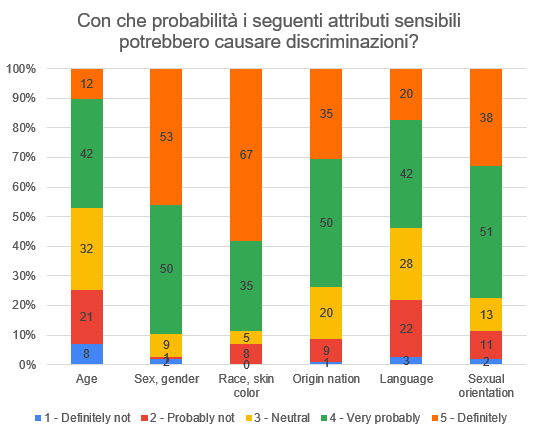
\includegraphics[width=360pt]{figure/data-analysis2/root1.png}
    \caption{Cause delle discriminazioni in termini di attributi sensibili}
    \label{im-a-root-1}
\end{figure}

\begin{figure}[h!]
    \centering
    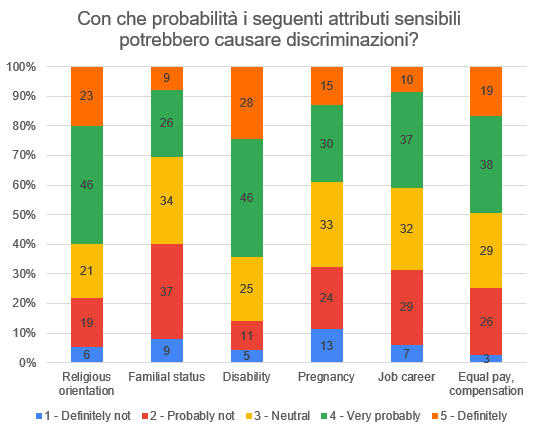
\includegraphics[width=360pt]{figure/data-analysis2/root2.png}
    \caption{Cause delle discriminazioni in termini di attributi sensibili}
    \label{im-a-root-2}
\end{figure}

Dai risultati ottenuti, secondo i partecipanti ci sono attributi sensibili che potrebbero essere causa di discriminazioni (figure \ref{im-a-root-1} e \ref{im-a-root-2}) con meno probabilità rispetto agli altri:
\begin{itemize}
    \item Lo stato familiare risulta essere causa di discriminazioni secondo 35 partecipanti (30,43\%);
    \item La gravidanza risulta essere causa di discriminazioni secondo 45 partecipanti (39,13\%);
    \item La carriera lavorativa risulta essere causa di discriminazioni secondo 47 partecipanti (40,86\%).
\end{itemize}

Attributi sensibili ritenuti particolarmente rilevanti, invece, sono i seguenti:
\begin{itemize}
    \item Il sesso e il gender risultano essere causa di discriminazioni secondo 103 partecipanti (89,56\%);
    \item La razza e il colore della pelle risultano essere causa di discriminazioni secondo 102 partecipanti (88,69\%);
    \item L'orientamento sessuale risulta essere causa di discriminazioni secondo 89 partecipanti (77,39\%);
    \item La nazione di origine risulta essere causa di discriminazioni secondo 85 partecipanti (73,91\%).
\end{itemize}
Riguardo gli altri attributi sensibili comunque è presente una buona fetta di partecipanti che pensano siano discriminatori: in generale, tali attributi sono valutati come causa di discriminazioni da circa il 50\% degli intervistati. È molto interessante, piuttosto, ciò che i partecipanti hanno espresso nella risposta aperta in cui si chiedeva se ci fossero altri attributi sensibili di cui non si era tenuto conto capaci di sollevare discriminazioni (figura \ref{im-a-root-3}): l'attributo più suggerito riguarda l'aspetto della persona (11 partecipanti), seguito dall'orientamento politico (8 partecipanti) e dallo stato sociale (6 partecipanti). Altri attributi comunque suggeriti abbastanza spesso (4, 5 partecipanti) sono lo stato finanziario, il livello di istruzione, il background culturale e lo stato di salute. Altre risposte, molto meno frequenti (1, 2 partecipanti) riguardano l'immigrazione, la partecipazione alla comunità LGBTQ+, hobby e passioni, comportamento personale e se una persona è vittima di bullismo.\\

\begin{figure}[h!]
    \centering
    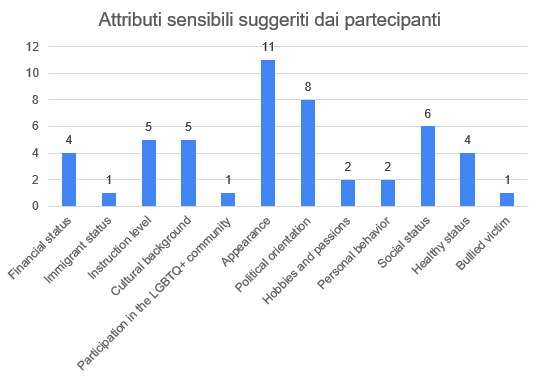
\includegraphics[width=360pt]{figure/data-analysis2/attroth.png}
    \caption{Attributi sensibili suggeriti dai partecipanti come causa di discriminazioni}
    \label{im-a-root-3}
\end{figure}

Sono stati messi in discussione anche aspetti legati al machine learning (figure \ref{im-a-root-4} e \ref{im-a-root-5}) per comprendere, secondo i partecipanti, potessero anch'essi essere causa di discriminazioni. Si ricorda che gli aspetti verranno elencati tramite identificativi stabiliti nella tabella \ref{table-root-id-1}. Analizzando le risposte, è sorta molta più indecisione rispetto alle risposte inerenti agli attributi sensibili: nel complesso, molti meno partecipanti hanno dato la massima certezza circa il fatto che un aspetto possa essere causa di discriminazione o meno rispetto agli attributi sensibili; inoltre, il numero di risposte neutrali complessivo è decisamente maggiore rispetto a quello legabile agli attributi sensibili.

\begin{figure}[h!]
    \centering
    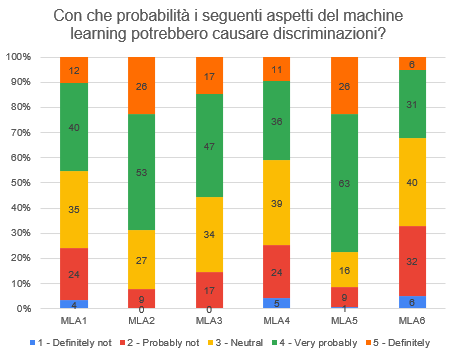
\includegraphics[width=360pt]{figure/data-analysis2/asp1.png}
    \caption{Cause delle discriminazioni in termini di aspetti del machine learning}
    \label{im-a-root-4}
\end{figure}
\begin{figure}[h!]
    \centering
    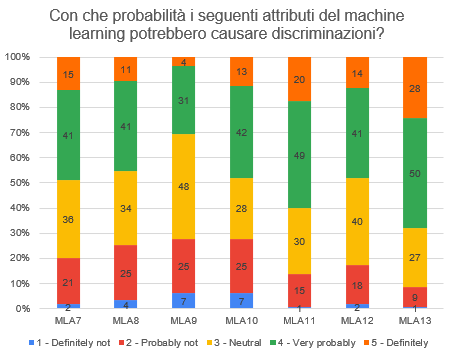
\includegraphics[width=360pt]{figure/data-analysis2/asp2.png}
    \caption{Cause delle discriminazioni in termini di aspetti del machine learning}
    \label{im-a-root-5}
\end{figure}

In ogni caso, dall'analisi dei risultati sono comunque sorti alcuni aspetti quali sono considerati da un buon numero di partecipanti come probabile causa di discriminazioni:
\begin{itemize}
    \item MLA5 - La presenza di feature sensibili nel dataset (77,39\%);
    \item MLA2 - Qualità dei dati presenti nel dataset (68,69\%);
    \item MLA13 - Svolgimento di attività di validazione su una partizione contenente solo soggetti discriminati (67,82\%).
\end{itemize}
I pareri dei partecipanti verso i rimanenti aspetti, invece, non dimostrano un grado di sicurezza soddisfacente circa il fatto possano essere causa di discriminazioni: in generale, le persone che si dimostrano concordi sul considerare i rimanenti aspetti una causa vanno dal 55\% dei partecipanti totali (MLA3 - Bilanciamento del dataset) fino a decrescere al 30\% di essi (MLA9 - Assegnazione degli hyperparameter).

\subsection{Classificazione in best e bad practice}
Ai partecipanti sono state poste alcune domande circa quelle che potrebbero, secondo loro, essere considerabili best o bad practice. Un primo quesito propone ai partecipanti una serie di practice, di cui alcune generiche per il machine learning, per comprendere quando siano considerabili best o bad approcciandole all'ambito fairness, e alcune direttamente più mirate agli aspetti legabili alla fairness. I successivi due quesiti, invece, chiedono ai partecipanti, in base alla loro esperienza lavorativa, eventuali altre practice di cui non si è tenuta considerazione durante la stesura del questionario.\\

Le practice proposte ai partecipanti sono le seguenti:
\begin{longtable}{| p{.30\textwidth} | p{.63\textwidth} |}
  \hline\textbf{\textit{Practice proposta}} & \textbf{\textit{Spiegazione}}
    \\ \hline
    \rowcolor{Gray!30}
    Svolgimento di attività di data balancing basate sulle feature sensibili
    &
    Avere un dataset non bilanciato non è un'opzione così remota. Si potrebbe, quindi, pensare che il dataset non bilanciato possa in qualche modo ricondurre a discriminazioni e che quest'ultime possano essere mitigate effettuando operazioni di bilanciamento dei dati concentrandosi sulle feature sensibili.
    \\ \hline
    Esecuzione del processo di training del modello principalmente sulle feature sensibili
    &
    Il training è il processo nel quale il modello impara a ragionare sui dati, quindi si potrebbe pensare di mitigare le discriminazioni andando ad agire sul modo in cui il modello apprende come svolgere le predizioni. Un'idea potrebbe essere quella di basare il training principalmente sulle feature sensibili.
    \\ \hline
    \rowcolor{Gray!30}
    Svolgimento di interview e focus groups al fine di elicitare requisiti inerenti la fairness
    &
    Le interview e i focus groups sono due buone metodologie per l'analisi e l'elicitazione dei requisiti. Si potrebbe pensare, quindi, di raccogliere requisiti, funzionali e non, che comprendano l'argomento fairness in modo da direzionare sin dagli albori la progettazione del sistema verso il rispetto della fairness.
     \\ \hline
    Utilizzo di combinazioni di modelli (ensemble learning)
    &
    L'uso di combinazioni di modelli permette di combinare le predizioni provenienti, appunto, da più modelli. Si potrebbe valutare, quindi, la combinazione di modelli classici con eventuali modelli orientati specificamente al rispetto della fairness, in modo che le predizioni tengano conto anche di quest'ultimo aspetto.
    \\ \hline
    \rowcolor{Gray!30}
    Tuning degli hyperparameter
    &
    Gli hyperparameter possono essere viste come variabili di configurazione, ad esempio nelle reti neutrali regolano il numero di hidden layer presenti. Tali parametri servono, quindi, a regolare il processo di learning e i loro valori possono essere variati in base a come il modello impara dai dati. Si potrebbe pensare che la loro regolazione in un particolar modo potrebbe andare ad influire sul rispetto della fairness.
    \\ \hline
    Selezione di uno specifico algoritmo di machine learning per il rispetto delle assunzioni legate alla fairness
    &
    La scelta di un algoritmo dipende dalle diverse assunzioni riguardanti il tipo di problema da risolvere e particolari caratteristiche tecniche del dataset. L'algoritmo deve rispettare le assunzioni che vengono sviluppate in fase di progettazione, quindi si potrebbe valutare lo sviluppo di assunzioni inerenti alla fairness in modo che l'algoritmo venga scelto tenendo conto di quest'ultimo aspetto.
    \\ \hline
    \rowcolor{Gray!30}
    Svolgimento di attività di validazione e testing su un dataset perfettamente bilanciato
    &
    Una volta costruito e allenato il modello, dovrà essere rigorosamente testato e validato tramite specifiche tecniche. Si propone di eseguire testing e validazione su un dataset bilanciato siccome con un dataset non bilanciato si potrebbero avere risultati poco realistici e non accurati.
     \\ \hline
    Considerare la fairness un aspetto prioritario durante la fase di analisi dei requisiti
    &
    Durante l'analisi e l'elicitazione dei requisiti può essere fondamentale trattare aspetti che possano ricondurre alla fairness: possono essere, quindi, discussi dal team di analisi per decidere se tenerne conto o meno, quanto rilevanti essi siano per il problema da affrontare. Considerando tali aspetti, si potrebbero mitigare le discriminazioni siccome il sistema verrebbe progettato tenendone conto.
    \\ \hline
    \rowcolor{Gray!30}
    Risoluzione di overfitting e underfitting tramite un particolare assegnamento ai pesi
    &
    Overfitting e underfitting sono due situazioni non gradite siccome in tali casi il modello fornisce predizioni irrealistiche. Si potrebbe ipotizzare un particolare assegnamento ai pesi in modo da risolvere tali situazioni, evitando predizioni che facciano troppo riferimento alle feature sensibili o che non ne tengano conto.
    \\ \hline
    Particolare assegnamento ai pesi in modo da rendere il modello più preciso nelle predizioni
    &
    Un modello che predice con un alto tasso di errori non è sicuramente soddisfacente. Potrebbe accedere che gli errori di predizione vengano confusi con le discriminazioni quando poi, in realtà, sono dovuti al fatto che il modello semplicemente possiede pesi errati. Pertanto, si potrebbe valutare un assegnamento più adeguato al fine di migliorare le predizioni.
    \\ \hline
    \rowcolor{Gray!30}
    Rimozione delle feature sensibili dal dataset
    &
    Un modo per mitigare le discriminazioni potrebbe consistere nella rimozione delle feature dal dataset, in modo da evitare che il modello le valuti durante le predizioni.
     \\ \hline
    Confronto di un modello che fa uso di attributi sensibili con un modello che non ne fa uso
    &
    Per questioni di monitoraggio, potrebbe essere utile svolgere un confronto tra un modello che predice tramite attributi sensibili con un altro che non ne fa uso. In tal modo, si potrebbero monitorare i risultati delle predizioni e comprendere se l'uso di attributi sensibili nella predizione ha un particolare impatto.
    \\ \hline
    \rowcolor{Gray!30}
    Esecuzione del processo di training su un dataset perfettamente bilanciato
    &
    Il training è il processo nel quale il modello impara a ragionare sui dati. Si propone di eseguire il training su un dataset bilanciato siccome con un dataset non bilanciato si potrebbero avere risultati poco realistici e non accurati.
     \\ \hline
    Svolgimento di attività di validazione su una partizione contenente solo soggetti discriminati
    &
    La validazione del modello potrebbe essere svolta solo su soggetti discriminati in modo da confermare se il modello svolge effettivamente delle discriminazioni su questi ultimi. Non si prevede, quindi, la validazione sugli altri soggetti.
    \\ \hline
    \rowcolor{Gray!30}
    Aggiunta di nuovi record nel dataset al fine di avvantaggiare gli individui discriminati
    &
    In generale, l'aggiunta di nuovi record nel dataset può portare ad un modello più preciso a patto che i dati siano qualitativamente buoni. Pertanto, si può pensare di inserire particolari dati al fine di avvantaggiare gli individui discriminati.
    \\ \hline
    Svolgimento di manutenzione ed evoluzione considerando i cambiamenti dei dati nel tempo
    &
    Il dataset può essere soggetto a cambiamenti nel tempo, quindi potrebbe essere necessario svolgere manutenzione ed evoluzione al fine di evitare che i nuovi dati possano provocare discriminazioni.
    \\ \hline
    \rowcolor{Gray!30}
    Assegnazione di valori casuali ai pesi del modello
    &
    L'assegnazione di valori casuali ai pesi del modello viene svolta per fare in modo tale che ad ogni sessione di training il modello adotti una tipologia di ragionamento diverso, così che tenga conto di aspetti non considerati nelle sessioni precedenti.
     \\ \hline
    \caption{Practice proposte e spiegazioni} % needs to go inside longtable environment
    \label{tab:myfirstlongtable}
\end{longtable}

I partecipanti hanno avuto la possibilità di indicare, secondo loro, se una practice possa essere ritenibile come best o bad tramite una scala in cui mostrassero quanto sicuri fossero della scelta. Per ottenere un giudizio complessivo circa la classificazione delle practice, tutte le risposte in cui è presente indecisione, eccetto le neutrali, verranno comunque conteggiate come positive o negative secondo quanto riportato dalla figura \ref{im-a-prac-1}. Si ricorda, infine, che le practice verranno elencate tramite identificativi stabiliti nella tabella \ref{table-root-id-2}.

\begin{figure}[h!]
    \centering
    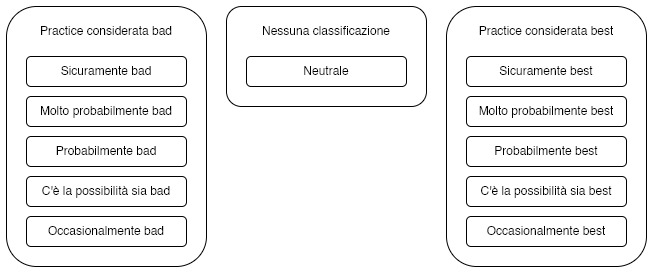
\includegraphics[width=400pt]{figure/data-analysis3/labelingbadbest.png}
    \caption{Classificazione delle risposte per le practice}
    \label{im-a-prac-1}
\end{figure}

Partendo dalla practice P1 (figura \ref{im-a-prac-2}), si nota che complessivamente si ha un quantitativo di risposte molto simile sia per la classificazione in bad che in best. Volendo andare più nel dettaglio, invece, si nota una leggera maggiore decisione verso la classificazione in bad practice, non creando comunque un dislivello significativo tra risposte bad e best. Si preferisce, quindi, non categorizzare la practice P1. Piuttosto, in una eventuale ripetizione dell'esperimento si potrebbero ottenere maggiori dati per tale practice ed effettuare una deduzione con maggiore criterio.

\begin{figure}[h!]
    \centering
    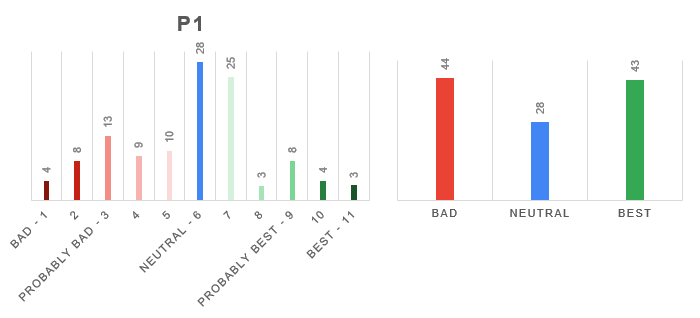
\includegraphics[width=1\textwidth]{figure/data-analysis3/P1.png}
    \caption{Risultati votazione practice P1}
    \label{im-a-prac-2}
\end{figure}

\begin{center}
    \begin{tcolorbox}[width=400pt, colframe=black, colback=Gray!30]
		\begin{minipage}{\textwidth}
			\textit{\faKey \textbf{ Risultato di ricerca 1}}\\
			È possibile affermare che lo svolgimento di attività di data balancing orientate principalmente al bilanciamento delle feature sensibili possa essere una practice corretta o meno a seconda della casistica riscontrata, siccome indicata sia come best che come bad practice.
		\end{minipage}
	\end{tcolorbox}
\end{center}

Riguardo la practice P2 (figura \ref{im-a-prac-3}), ha ricevuto un buon numero di risposte per poterla classificare come bad practice (61 partecipanti complessivi) rispetto alla classificazione in best (44 partecipanti complessivi). In particolare, andando nel dettaglio, ci sono state risposte indicanti decisamente maggiore certezza circa il fatto che sia una bad practice: la maggior parte dei voti inerente alla classificazione best proviene dal valore 7 (25 partecipanti), il che è un valore che esprime molta incertezza. Piuttosto, sono in 25 i partecipanti complessivi che hanno votato da 1 a 3, indicante una buona sicurezza nel fatto che la practice sia bad, rispetto ai 15 partecipanti complessivi che hanno votato da 9 a 11.

\begin{figure}[h!]
    \centering
    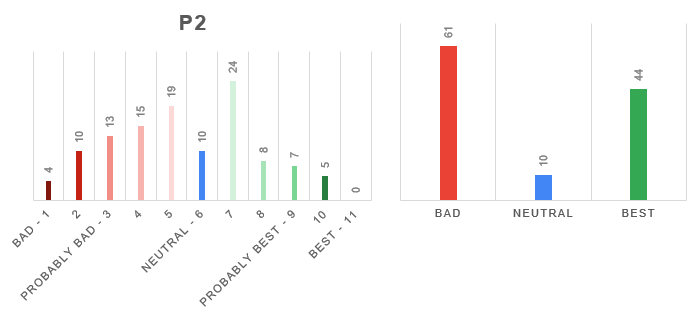
\includegraphics[width=1\textwidth]{figure/data-analysis3/P2.png}
    \caption{Risultati votazione practice P2}
    \label{im-a-prac-3}
\end{figure}

\begin{center}
    \begin{tcolorbox}[width=400pt, colframe=black, colback=Gray!30]
		\begin{minipage}{\textwidth}
			\textit{\faKey \textbf{ Risultato di ricerca 2}}\\
			È possibile affermare che basare l'addestramento del modello, quindi la fase di training, principalmente sugli attributi sensibili capaci di scatenare discriminazioni sia una \textbf{bad practice}, dato che le risposte appartenenti alla categoria "bad" superano di 20 quelle della categoria "best".
		\end{minipage}
	\end{tcolorbox}
\end{center}

Parlando della practice P3 (figura \ref{im-a-prac-4}), ha ricevuto moltissimi voti circa la considerabilità in best practice (64 partecipanti complessivi) rispetto alla classificazione in bad (32 partecipanti complessivi). Analizzando nel dettaglio si conferma la classificazione in best practice siccome si è ricevuto un buon numero di voti che vanno da 9 a 11 (25 partecipanti complessivi). In pochi (7 partecipanti complessivi), invece, hanno preferito classificarla come bad practice dando un voto che va da 1 a 3.

\begin{figure}[h!]
    \centering
    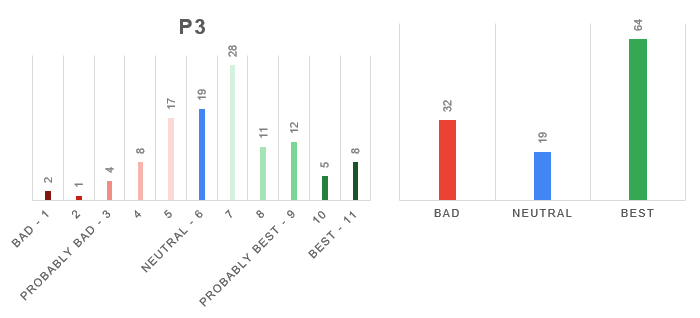
\includegraphics[width=1\textwidth]{figure/data-analysis3/P3.png}
    \caption{Risultati votazione practice P3}
    \label{im-a-prac-4}
\end{figure}

\begin{center}
    \begin{tcolorbox}[width=400pt, colframe=black, colback=Gray!30]
		\begin{minipage}{\textwidth}
			\textit{\faKey \textbf{ Risultato di ricerca 3}}\\
			È possibile affermare che lo svolgimento di interview e di focus group con l'obiettivo di elicitare requisiti che abbiano a che fare con la fairness sia una \textbf{best practice}, dato che le risposte appartenenti alla categoria "best" superano di 32 quelle della categoria "bad".
		\end{minipage}
	\end{tcolorbox}
\end{center}

La practice P4 (figura \ref{im-a-prac-5}) riporta anch'essa una maggiore preferenza verso la classificazione in best practice (63 partecipanti complessivi). È interessante, per tale pratica, sapere che osservando i dettagli sono state fornite molte risposte indicanti molta sicurezza nella classificazione in best practice: difatti, ben 26 partecipanti complessivi hanno dato un voto tra 9 e 11, mentre quasi nessuno ha dato un voto tra 1 e 3 (5 partecipanti complessivi).

\begin{figure}[h!]
    \centering
    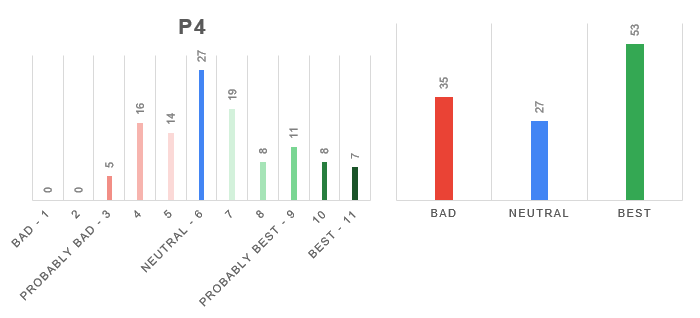
\includegraphics[width=1\textwidth]{figure/data-analysis3/P4.png}
    \caption{Risultati votazione practice P4}
    \label{im-a-prac-5}
\end{figure}

\begin{center}
    \begin{tcolorbox}[width=400pt, colframe=black, colback=Gray!30]
		\begin{minipage}{\textwidth}
			\textit{\faKey \textbf{ Risultato di ricerca 4}}\\
			È possibile affermare che l'uso di più modelli per lo svolgimento di una predizione sia una \textbf{best practice}, dato che le risposte appartenenti alla categoria "best" superano di 18 quelle della categoria "bad", le quali mostrano un alto tasso di incertezza.
		\end{minipage}
	\end{tcolorbox}
\end{center}

Discorso analogo per le practice P5 e P6 (figure \ref{im-a-prac-6} e \ref{im-a-prac-7}): le risposte mostrano una buona sicurezza da parte dei partecipanti nel classificare la practice come best, visto il numero di voti che vanno da 9 a 11 (25 partecipanti complessivi per P5, 22 partecipanti complessivi per P6). Piccola nota riguarda il numero di risposte neutrali, il quale è abbastanza alto per la practice P5: 32 partecipanti hanno preferito non classificare P5 come best o come bad.

\begin{figure}[h!]
    \centering
    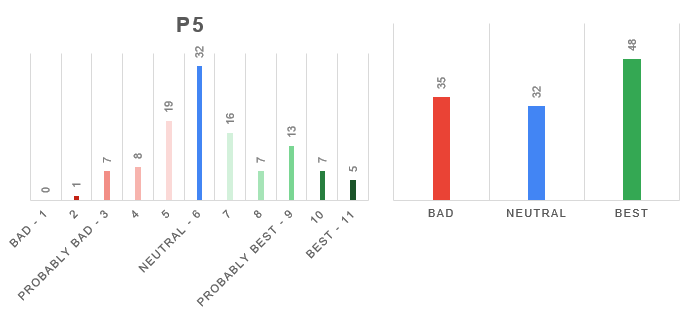
\includegraphics[width=1\textwidth]{figure/data-analysis3/P5.png}
    \caption{Risultati votazione practice P5}
    \label{im-a-prac-6}
\end{figure}

\begin{figure}[h!]
    \centering
    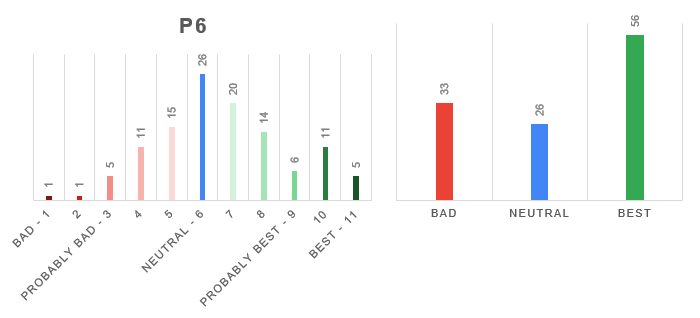
\includegraphics[width=1\textwidth]{figure/data-analysis3/P6.png}
    \caption{Risultati votazione practice P6}
    \label{im-a-prac-7}
\end{figure}

\begin{center}
    \begin{tcolorbox}[width=400pt, colframe=black, colback=Gray!30]
		\begin{minipage}{\textwidth}
			\textit{\faKey \textbf{ Risultato di ricerca 5}}\\
			È possibile affermare che la regolazione dei valori degli hyperparameter e la selezione di un algoritmo di machine learning che rispetti le assunzioni circa gli aspetti fairness siano entrambe \textbf{best practice}, dato che le risposte appartenenti alla categoria "best" superano quelle della categoria "bad" rispettivamente di 13 e 23 voti. Inoltre, diversi partecipanti hanno espresso una preferenza neutrale inerente alla regolazione dei valori degli hyperparameter.
		\end{minipage}
	\end{tcolorbox}
\end{center}

Le practice P7 e P8 (figure \ref{im-a-prac-8} e \ref{im-a-prac-9}), invece, delineano una massiccia preferenza verso la categorizzazione in best practice (71 partecipanti complessivi per P7, 67 partecipanti complessivi per P8) con una differenza di voti tra categorizzazione in best e bad rispettivamente di 38 e 37 voti. Sono presenti molte risposte che esprimono molta sicurezza nella classificazione in best, difatti l'intervallo di voti da 9 a 11 è decisamente concentrato (29 partecipanti complessivi per P7, 32 partecipanti complessivi per P8). La practice P8 in particolare ha ricevuto un ottimo numero di voti indicanti la massima sicurezza circa la classificazione in best practice (14 partecipanti), come anche P7 che ne totalizza qualcuno in meno (10 partecipanti).

\begin{figure}[h!]
    \centering
    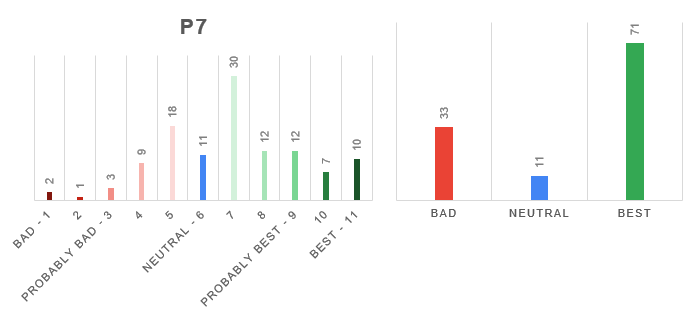
\includegraphics[width=1\textwidth]{figure/data-analysis3/P7.png}
    \caption{Risultati votazione practice P7}
    \label{im-a-prac-8}
\end{figure}
\begin{figure}[h!]
    \centering
    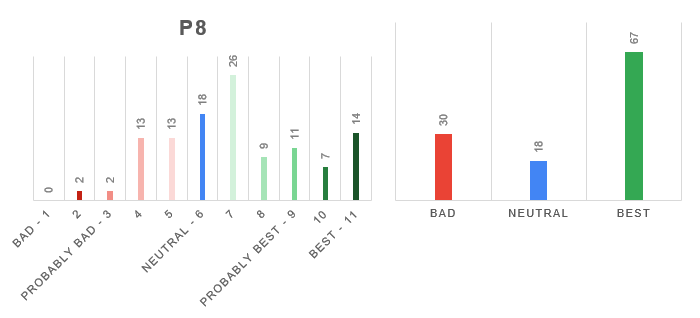
\includegraphics[width=1\textwidth]{figure/data-analysis3/P8.png}
    \caption{Risultati votazione practice P8}
    \label{im-a-prac-9}
\end{figure}

\begin{center}
    \begin{tcolorbox}[width=400pt, colframe=black, colback=Gray!30]
		\begin{minipage}{\textwidth}
			\textit{\faKey \textbf{ Risultato di ricerca 6}}\\
			È possibile affermare che validare e testare un modello su un dataset perfettamente bilanciato e considerare la fairness un aspetto prioritario durante l'analisi dei requisiti siano entrambe \textbf{best practice}, dato che le risposte appartenenti alla categoria "best" sono molto più evidenti di quelle della categoria "bad", con una rispettiva differenza di 38 e 37 voti.
		\end{minipage}
	\end{tcolorbox}
\end{center}

Anche le practice P9 e P10 (figure \ref{im-a-prac-10} e \ref{im-a-prac-11}) risultano avere una buona preferenza di voti verso la classificazione in best practice (56 partecipanti complessivi per P9, 59 partecipanti complessivi per P10); in particolare, P10 ha ottenuto maggiore sicurezza nell'intervallo di voti da 9 a 11 (23 partecipanti complessivi) rispetto a P9 (16 partecipanti complessivi) che dimostra una leggera incertezza tramite il numero di voti 7 e 8 leggermente alto, ma non rilevante ai fini della classificazione svolta.

\begin{figure}[h!]
    \centering
    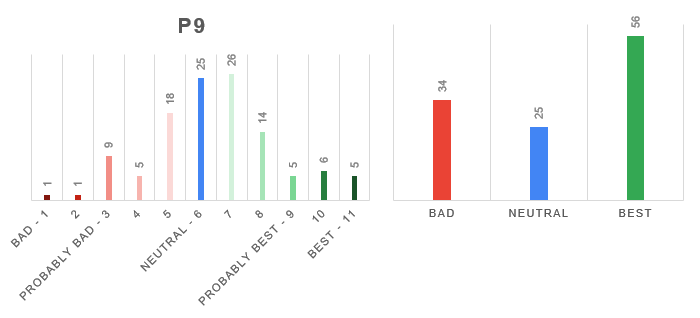
\includegraphics[width=1\textwidth]{figure/data-analysis3/P9.png}
    \caption{Risultati votazione practice P9}
    \label{im-a-prac-10}
\end{figure}
\begin{figure}[h!]
    \centering
    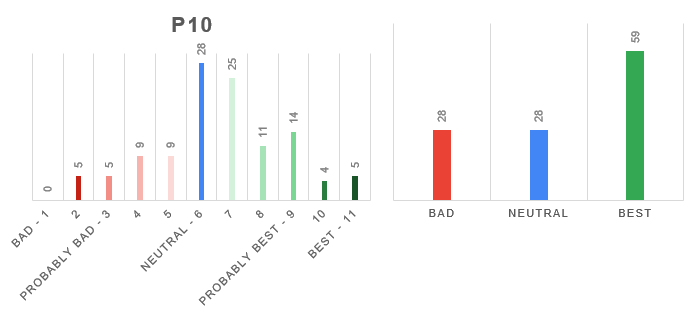
\includegraphics[width=1\textwidth]{figure/data-analysis3/P10.png}
    \caption{Risultati votazione practice P10}
    \label{im-a-prac-11}
\end{figure}

\begin{center}
    \begin{tcolorbox}[width=400pt, colframe=black, colback=Gray!30]
		\begin{minipage}{\textwidth}
			\textit{\faKey \textbf{ Risultato di ricerca 7}}\\
			È possibile affermare che assegnare particolari valori ai pesi in modo da risolvere situazioni di overfitting e underfitting e in modo da rendere il modello più accurato durante le sue previsioni siano entrambe \textbf{best practice}, dato che le risposte appartenenti alla categoria "best" superano quelle della categoria "bad" rispettivamente di 22 e 31 voti.
		\end{minipage}
	\end{tcolorbox}
\end{center}

La practice P11 (figura \ref{im-a-prac-12}), invece, ha ricevuto un alto numero di voti che riguardassero la classificazione in bad practice (65 partecipanti complessivi). Andando nel dettaglio, sono molti i voti esprimenti sicurezza circa la classificazione bad: ben 26 partecipanti complessivi hanno espresso come propria preferenza un voto che va da 1 a 3. In generale, comunque, la stragrande maggioranza dei voti tende a riferire sempre alla classificazione bad.

\begin{figure}[h!]
    \centering
    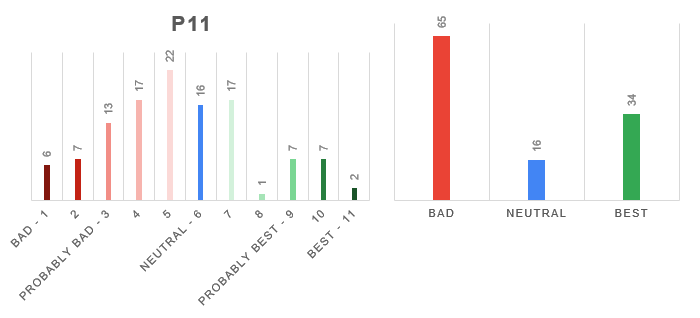
\includegraphics[width=1\textwidth]{figure/data-analysis3/P11.png}
    \caption{Risultati votazione practice P11}
    \label{im-a-prac-12}
\end{figure}

\begin{center}
    \begin{tcolorbox}[width=400pt, colframe=black, colback=Gray!30]
		\begin{minipage}{\textwidth}
			\textit{\faKey \textbf{ Risultato di ricerca 8}}\\
			È possibile affermare che la rimozione delle feature sensibili dal dataset, in modo da evitare che il training tenga conto di tali attributi, sia una \textbf{bad practice}, dato che le risposte appartenenti alla categoria "bad" superano di 31 quelle della categoria "best".
		\end{minipage}
	\end{tcolorbox}
\end{center}

Molto interessante analizzare anche P12 (figura \ref{im-a-prac-13}), un'altra practice la cui classificazione non è resa possibile a causa della leggera differenza tra risposte che la classificano come best e risposte che la classificano come bad. Anche gli intervalli in cui si esprime maggiore sicurezza sono stati votati da diversi partecipanti, difatti 15 partecipanti complessivi hanno dato un voto da 1 a 3, mentre 19 partecipanti hanno dato un voto da 9 a 11.

\begin{figure}[h!]
    \centering
    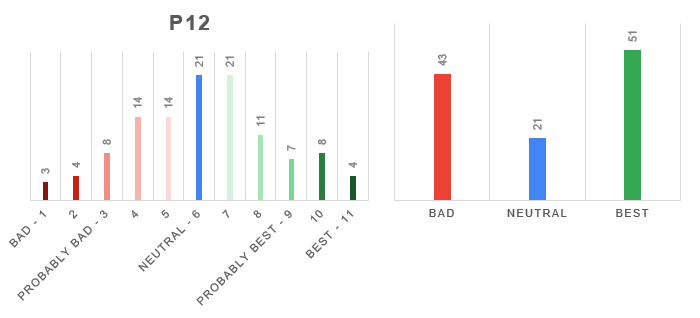
\includegraphics[width=1\textwidth]{figure/data-analysis3/P12.png}
    \caption{Risultati votazione practice P12}
    \label{im-a-prac-13}
\end{figure}

\begin{center}
    \begin{tcolorbox}[width=400pt, colframe=black, colback=Gray!30]
		\begin{minipage}{\textwidth}
			\textit{\faKey \textbf{ Risultato di ricerca 9}}\\
			È possibile affermare che paragonare un modello che fa uso degli attributi sensibili per svolgere le predizioni con uno di cui non ne fa uso possa essere una practice corretta o meno a seconda della casistica riscontrata, siccome indicata sia come best che come bad practice.
		\end{minipage}
	\end{tcolorbox}
\end{center}

La practice P13 (figura \ref{im-a-prac-14}), invece, ha riscontrato un ottimo numero di risposte in cui si esprime una buona sicurezza circa il fatto che sia classificabile come best: nell'intervallo di voti da 9 a 11 si sono espressi 28 partecipanti complessivi, di cui 11 hanno espresso la massima sicurezza. A testimone di ciò, anche le risposte complessive contrassegnate con "best" (63 partecipanti complessivi) risultano essere decisamente maggiori di quelle contrassegnate con "bad" (31 partecipanti complessivi).

\begin{figure}[h!]
    \centering
    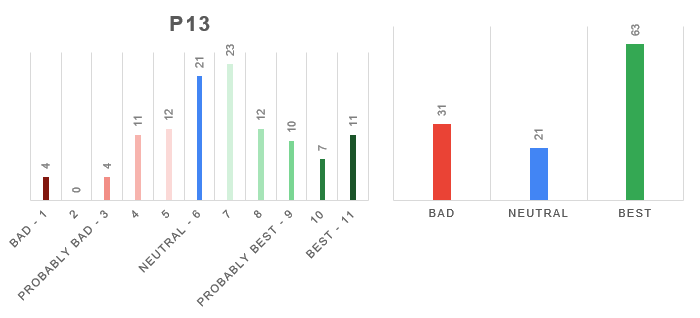
\includegraphics[width=1\textwidth]{figure/data-analysis3/P13.png}
    \caption{Risultati votazione practice P13}
    \label{im-a-prac-14}
\end{figure}

\begin{center}
    \begin{tcolorbox}[width=400pt, colframe=black, colback=Gray!30]
		\begin{minipage}{\textwidth}
			\textit{\faKey \textbf{ Risultato di ricerca 10}}\\
			È possibile affermare che effettuare il training del modello su un dataset ben bilanciato sia una \textbf{best practice}, dato che le risposte appartenenti alla categoria "best" superano di 32 quelle della categoria "bad".
		\end{minipage}
	\end{tcolorbox}
\end{center}

P14 e P15 (figure \ref{im-a-prac-15} e \ref{im-a-prac-16}), invece, sono due pratiche in particolare i cui voti predominanti fanno sicuramente riferimento al fatto che siano considerabili bad practice (rispettivamente 56 partecipanti complessivi e 60 partecipanti complessivi), ma allo stesso tempo sono presenti voti che esprimono una buona sicurezza circa il fatto che possano essere best practice, indicati nell'intervallo da 9 a 11 (rispettivamente 12 partecipanti e 10 partecipanti). Senza ombra di dubbio sono deducibili essere bad practice, ma c'è comunque qualche partecipante che, evidentemente, gradirebbe ritenerle best practice in particolari occasioni.

\begin{figure}[h!]
    \centering
    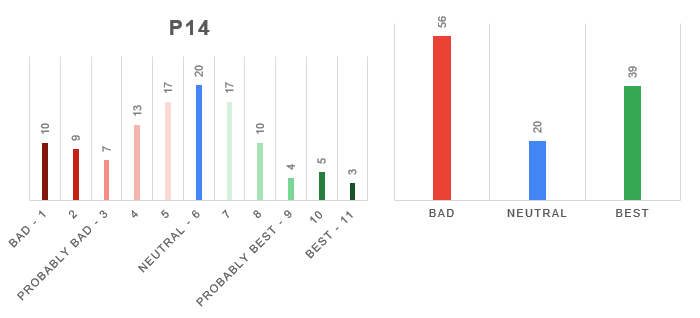
\includegraphics[width=1\textwidth]{figure/data-analysis3/P14.png}
    \caption{Risultati votazione practice P14}
    \label{im-a-prac-15}
\end{figure}
\begin{figure}[h!]
    \centering
    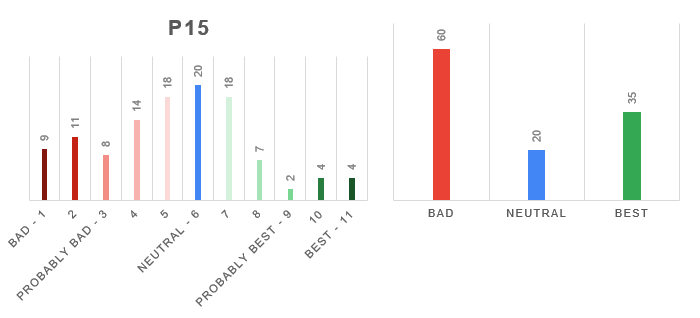
\includegraphics[width=1\textwidth]{figure/data-analysis3/P15.png}
    \caption{Risultati votazione practice P15}
    \label{im-a-prac-16}
\end{figure}

\begin{center}
    \begin{tcolorbox}[width=400pt, colframe=black, colback=Gray!30]
		\begin{minipage}{\textwidth}
			\textit{\faKey \textbf{ Risultato di ricerca 11}}\\
			È possibile affermare che validare un modello sulla base di una partizione contenente solo soggetti discriminati e aggiungere nuovi record nel dataset in modo da far preferire, al modello, i soggetti discriminati siano entrambe \textbf{bad practice}, dato che le risposte appartenenti alla categoria "bad" superano quelle della categoria "best" rispettivamente di 17 e 25 voti. Pertanto, sono presenti dei partecipanti che sarebbero comunque disposte ad utilizzarle.
		\end{minipage}
	\end{tcolorbox}
\end{center}

La practice P16 (figura \ref{im-a-prac-17}) ha ottenuto un ottimo numero di risposte per la quale la classificano come best (66 partecipanti complessivi). Analizzando le risposte nel dettaglio, però, si denota molta indecisione dato il gran numero di voti pari a 7 (34 partecipanti). Tale dettaglio è comunque irrilevante alla classificazione siccome sono comunque presenti diversi voti rientranti nell'intervallo da 9 a 11 (22 partecipanti complessivi).

\begin{figure}[h!]
    \centering
    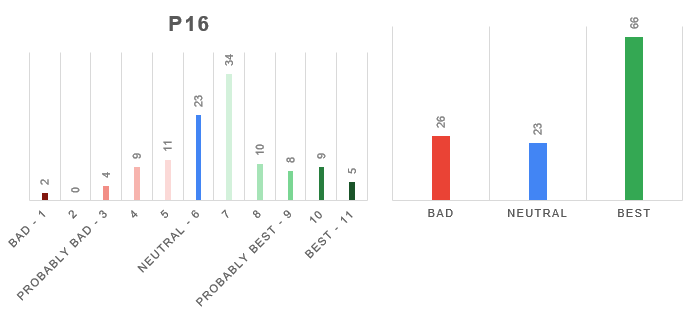
\includegraphics[width=1\textwidth]{figure/data-analysis3/P16.png}
    \caption{Risultati votazione practice P16}
    \label{im-a-prac-17}
\end{figure}

\begin{center}
    \begin{tcolorbox}[width=400pt, colframe=black, colback=Gray!30]
		\begin{minipage}{\textwidth}
			\textit{\faKey \textbf{ Risultato di ricerca 12}}\\
			È possibile affermare che svolgere manutenzione sul sistema realizzato o comunque svolgere evoluzione tenendo conto di eventuali variazioni dei dati nel tempo sia una \textbf{best practice}, dato che le risposte appartenenti alla categoria "best" sono molto più evidenti di quelle della categoria "bad", con una differenza di 40 voti.
		\end{minipage}
	\end{tcolorbox}
\end{center}

Infine, la practice P17 (figura \ref{im-a-prac-18}) ha ricevuto un buon numero di risposte per poterla classificare come bad practice (66 partecipanti complessivi) rispetto alla classificazione in best (27 partecipanti complessivi). In particolare, andando nel dettaglio, c'è un numero decisamente rilevante di partecipanti che hanno dato la massima certezza alla classificazione bad (16 partecipanti); contando l'intervallo di voti da 1 a 3, ben 38 partecipanti complessivi hanno dimostrato un buon grado di certezza circa la classificazione.

\begin{figure}[h!]
    \centering
    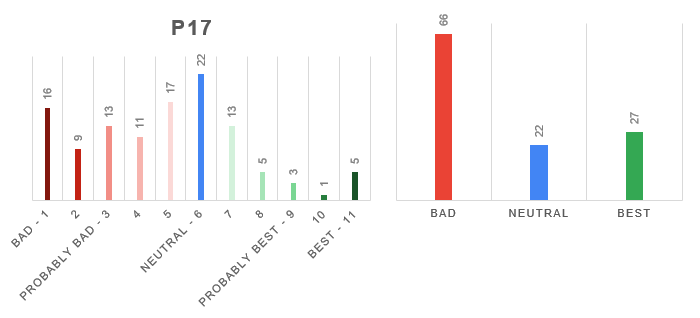
\includegraphics[width=1\textwidth]{figure/data-analysis3/P17.png}
    \caption{Risultati votazione practice P17}
    \label{im-a-prac-18}
\end{figure}

\begin{center}
    \begin{tcolorbox}[width=400pt, colframe=black, colback=Gray!30]
		\begin{minipage}{\textwidth}
			\textit{\faKey \textbf{ Risultato di ricerca 13}}\\
			È possibile affermare l'assegnazione di valori randomici ai pesi del modello che cambino da una sessione di training all'altra sia una \textbf{bad practice}, dato che le risposte appartenenti alla categoria "bad" sono molto più evidenti di quelle della categoria "best", con una differenza di 39 voti.
		\end{minipage}
	\end{tcolorbox}
\end{center}

Infine, come anticipato, ai partecipanti sono state somministrate anche due domande aperte in cui si chiedeva se fossero a conoscenza di altre best o bad practice, in modo da arricchire il catalogo. Ebbene, buona parte delle risposte concorda con le pratiche riportate, mentre qualche partecipante propone consigli generici come i seguenti:
\begin{itemize}
    \item Controllare i dati che il software colleziona, quindi revisionarli periodicamente;
    \item Svolgere dei meeting per discutere delle eventuali discriminazioni del sistema;
    \item Creare diversi scenari di testing.
\end{itemize}
Dalle risposte ottenute, purtroppo, non è possibile ricavare nuove pratiche.

\section{Discussioni e implicazioni}
\subsection{Cause delle discriminazioni}
Dall'analisi dei dati è risultato molto interessante conoscere quali, secondo la maggioranza dei partecipanti, potessero essere le cause scatenanti le discriminazioni e quanto fossero ritenute importanti. A parte qualche eccezione, quasi tutti gli attributi sensibili proposti sono stati ritenuti come causa di discriminazione, dando molta rilevanza agli attributi socialmente più discussi come il sesso, il gender, la razza, il colore della pelle e l'orientamento sessuale. Nonostante tali attributi siano oggigiorno ampiamente discussi, alcuni partecipanti pensano comunque non possano essere causa di discriminazioni, ma sono una minoranza rispetto al totale. Diversi partecipanti, inoltre, hanno preferito esplicitare altri attributi sensibili che potrebbero essere causa di discriminazioni ed è sorta una certa rilevanza verso l'aspetto fisico e l'orientamento politico, proposti da un buon numero di partecipanti. In ogni caso, gli attributi che possano creare discriminazioni sono molteplici ed è difficile valutarli tutti, sopratutto durante la pianificazione di un sistema di machine learning dato che i pareri circa le cause delle discriminazioni sono comunque soggettivi. Sicuramente possono esserci attributi maggiormente discussi nella società attuale e, di conseguenza, attribuibili subito a cause di discriminazione, ma l'analisi evidenzia il fatto che molte persone non ritengono discriminatori attributi come lo stato familiare \cite{familial-status-disc} e la gravidanza \cite{pregnancy-disc}. Sicuramente sarà dovuto anche al fatto che tali attributi sono meno discussi quando si parla di discriminazioni e di opportunità non eque, quindi sarebbe opportuno sensibilizzare le persone anche verso gli attributi di cui si parla meno in modo tale da essere consapevoli che anche quelli potrebbero creare situazioni in cui la persona si senta discriminata e non al pari degli altri.\\
Riguardo gli aspetti legati al machine learning, invece, è stata data forte rilevanza agli aspetti legati al dataset, come la presenza di feature sensibili, la qualità dei dati e i contenuti delle partizioni sul dataset, ma non mancano gli aspetti legati al modello. Andando nel dettaglio, le risposte dei candidati sono state più incerte rispetto a quelle fornite per gli attributi sensibili: ciò potrebbe essere dovuto al fatto che l'argomento fairness è ancora oggetto di studi e ancora non è definito, dalla letteratura, quali potrebbero essere le effettive cause e soluzioni per mitigare le discriminazioni. Nonostante l'insicurezza, le risposte complessive fornite risultano comunque essere coerenti con ciò che si è analizzato riguardo le practice: ad esempio, molti degli aspetti del machine learning ritenuti cause di discriminazioni fanno riferimento ai dati del dataset, il che è oggetto di diverse practice come quelle inerenti al bilanciamento dei dati (classificate come best) e alla rimozione delle feature sensibili (classificata come bad).

\subsection{Classificazione in best e bad practice}
\subsubsection{Best practice}
Dall'analisi dei dati si è riusciti a classificare un elenco di best practice, quindi rappresentanti tecniche e procedure le quali sarebbero buona norma da seguire. In primis, sono risultati essere best practice il considerare la fairness un aspetto cruciale durante l'analisi dei requisiti e lo svolgimento di interview e di focus group mirati all'elicitazione di requisiti fair, quindi requisiti che vadano a descrivere aspetti legati alla fairness che dovranno essere rispettati durante l'implementazione. Tali practice potrebbero essere accomunate siccome entrambe trattano la fase di analisi, quindi tutte procedure e azioni preliminari al design del sistema. Trattare la fairness in una fase preliminare può essere di cruciale importanza siccome si progetta il sistema in modo tale che rispetti particolari vincoli fair, quindi la mitigazione delle discriminazioni potrebbe avvenire sin dalla progettazione. È sicuramente una practice da approfondire siccome si potrebbero pensare, in un futuro sviluppo, la realizzazione di uno standard che definisca una serie di procedure da seguire in fase di analisi per far sì che le discriminazioni vengano mitigate quanto possibile.

\begin{center}
    \begin{tcolorbox}[width=400pt, colframe=black, colback=Gray!10]
			\begin{minipage}{\textwidth}
				\textit{\faCaretSquareORight  \textbf{ Implicazione 1}}\\
		     Si potrebbe pensare di discutere aspetti inerenti alla fairness in fase di analisi per poi elicitare requisiti fair oriented, mitigando quanto possibile le discriminazioni ben prima dello sviluppo del sistema intelligente. Si potrebbe pensare di realizzare uno standard da seguire a riguardo.
			\end{minipage}
	\end{tcolorbox}
\end{center}

Altre due practice ritenute "best" che potrebbero essere accomunate riguardano il training, la validazione e il testing del modello su un dataset bilanciato, in modo da realizzare un'unica best practice che riguardi l'intero sviluppo del modello. Avere un dataset bilanciato significa che ogni possibile output deve poter essere rappresentato dallo stesso numero, o simile, di individui. Nel caso si abbia un dataset sbilanciato, risulta essere best practice effettuare particolari operazioni per bilanciarlo, in modo che il training, la validazione e il testing del modello vengano eseguiti con particolare affidabilità. Avere un dataset sbilanciato potrebbe effettivamente essere un sintomo di discriminazione, dato che particolari individui appartenenti ad un determinato gruppo sarebbero quantitativamente inferiori rispetto a quelli di un altro gruppo. Volendo fare un esempio, un dataset in cui il colore della pelle è una feature sensibile dovrebbe avere lo stesso, o simile, numero di soggetti bianchi e di soggetti neri, altrimenti il modello potrebbe preferire una delle due categorie.

\begin{center}
    \begin{tcolorbox}[width=400pt, colframe=black, colback=Gray!10]
			\begin{minipage}{\textwidth}
				\textit{\faCaretSquareORight  \textbf{ Implicazione 2}}\\
		     Avere un dataset sbilanciato potrebbe essere sintomo di discriminazione a causa della prevalenza di un gruppo di dati rispetto ad un altro; pertanto, le fasi di training, validazione e testing andrebbero svolte su un dataset bilanciato, in cui i gruppi di dati sono tra loro considerati alla pari.
			\end{minipage}
	\end{tcolorbox}
\end{center}

Altra best practice riguardante il dataset consiste nel fatto che, con il passare del tempo, i dati possono cambiare e ciò può richiedere l'esecuzione di manutenzione o evoluzione per il sistema intelligente. Un cambiamento dei dati potrebbe portare alla nascita di discriminazioni nel caso vengano aggiunte feature sensibili o vengano aggiunti particolari individui che vadano a sbilanciare il dataset: in entrambi i casi, sarebbe necessario svolgere un minimo di manutenzione o evoluzione sul modello.

\begin{center}
    \begin{tcolorbox}[width=400pt, colframe=black, colback=Gray!10]
			\begin{minipage}{\textwidth}
				\textit{\faCaretSquareORight  \textbf{ Implicazione 3}}\\
		     I cambiamenti del modello dovrebbero stare al passo dei cambiamenti del dataset, soprattutto se strutturali: pertanto, è considerabile best practice l'esecuzione di manutenzione o evoluzione in modo tale che il modello venga adattato ai cambiamenti apportati sul dataset.
			\end{minipage}
	\end{tcolorbox}
\end{center}

Un altro aspetto fondamentale sembra essere l'assegnamento dei pesi del modello. Riguardo ciò, sono state proposte due best practice inerenti all'assegnazione di particolari valori ai pesi del modello in modo tale che le predizioni siano più accurate, evitando il fenomeno dell'underfitting, ma non al punto da ricadere in una situazione di overfitting. Insomma, viene proposto di raffinare il modello tramite i pesi senza esagerare, senza farlo diventare così preciso al punto da creare overfitting. Ciò ha molto senso siccome le situazioni di overfitting, in casi in cui sono presenti feature sensibili nel dataset, potrebbero permettere al modello di svolgere predizioni troppo impuntate sugli attributi sensibili del soggetto: da qui, potrebbero nascere discriminazioni. Volendo fare un esempio, si possiede un dataset di criminali americani e molti di essi si ipotizza siano neri: se il modello si impunta troppo sul colore della pelle, stabilirà che ogni soggetto nero estraneo al dataset sarà un criminale, il che è più che scorretto dato che il colore della pelle non fa di una persona un delinquente.

\begin{center}
    \begin{tcolorbox}[width=400pt, colframe=black, colback=Gray!10]
			\begin{minipage}{\textwidth}
				\textit{\faCaretSquareORight  \textbf{ Implicazione 4}}\\
		     Raffinare i valori dei pesi di un modello non solo evita le situazioni di underfitting, quindi situazioni in cui le predizioni hanno un alto tasso di errori, ma rende il modello stesso più preciso e più affidabile. Tuttavia, è bene evitare le situazioni di overfitting siccome potrebbero dar vita a discriminazioni nel caso il modello inizi a fare troppo riferimento alle feature sensibili. Pertanto, è buona pratica non raffinare ulteriormente i valori dei pesi se c'è il rischio di cadere in situazioni di overfitting.
			\end{minipage}
	\end{tcolorbox}
\end{center}

In ogni caso, può capitare che l'assegnazione di valori ai pesi raffini troppo il modello e si ricada in una situazione di overfitting. Nel caso ciò accada, potrebbe essere di buon aiuto regolare gli hyperparameter, i quali sono variabili che impostano diverse caratteristiche del modello. Se si parla di reti neurali, ad esempio, si possono usare gli hyperparameter per regolare il numero di hidden layer ed evitare situazioni di overfitting. Ovviamente gli hyperparameter non risolvono solo le situazioni di overfitting, in generale caratterizzano diversi aspetti del modello risolvendo, se impostati correttamente, conseguenze date da un'impostazione erronea del modello. Pertanto, la classificazione in best practice del tuning degli hyperparameter è in linea con quanto detto.

\begin{center}
    \begin{tcolorbox}[width=400pt, colframe=black, colback=Gray!10]
			\begin{minipage}{\textwidth}
				\textit{\faCaretSquareORight  \textbf{ Implicazione 5}}\\
		     Una scorretta configurazione del modello può portare a situazioni capaci di generare discriminazioni durante le predizioni: per far fronte a ciò, è necessario regolare i valori degli hyperparameter in modo da trovare i valori di configurazione più adatti al modello riducendo casistiche critiche che porterebbero ad eventi unfair.
			\end{minipage}
	\end{tcolorbox}
\end{center}

Infine, è stata proposta una practice che riguardasse la scelta dell'algoritmo di learning in base alle supposizioni svolte in fase di design del modello. Non sempre un modello può soddisfare tutte le supposizioni dedotte dal team di analisi, quindi può essere necessario utilizzare più modelli durante le predizioni, altra practice reputata "best" dai partecipanti. L'uso di più modelli permette di generare un esito ricavato da più predizioni, combinando gli esiti di ognuna. Tali practice possono essere combinate dato che in fase di progettazione potrebbero essere realizzate delle supposizioni che riguardino aspetti della fairness, quindi si potrebbe realizzare un modello che le rispetti e che predica insieme ad altri modelli che rispetteranno, a loro volta, altre supposizioni. Questa è una proposta di utilizzo che potrebbe essere realizzata nella casistica in cui si abbiano assunzioni circa aspetti legati alla fairness e aspetti che non la riguardino, ma l'uso di più modelli potrebbe benissimo comportare altri vantaggi: anche queste practice andrebbero sicuramente approfondite in uno studio futuro.

\begin{center}
    \begin{tcolorbox}[width=400pt, colframe=black, colback=Gray!10]
			\begin{minipage}{\textwidth}
				\textit{\faCaretSquareORight  \textbf{ Implicazione 6}}\\
		     Nel caso siano state svolte molte assunzioni sul modello, tra cui assunzioni inerenti agli aspetti fair, potrebbe essere un'idea utilizzare più modelli in modo da rispettare ogni assunzione realizzata. L'uso di più modelli comporta la combinazione dei risultati di predizione, quindi si otterrebbe un risultato che tenga conto anche delle assunzioni fair svolte per far fronte alle discriminazioni.
			\end{minipage}
	\end{tcolorbox}
\end{center}

\subsubsection{Bad practice}
Dall'analisi dei dati si è riusciti a classificare un elenco di bad practice, quindi rappresentanti tecniche e procedure le quali sarebbe meglio non seguire. Una prima practice categorizzata come "bad" riguarda il training del modello principalmente sulle feature sensibili. Probabilmente la classificazione in "bad" può essere giustificata dal fatto che basare il training principalmente sulle feature sensibili comporterebbe predizioni da parte del modello svolte dando maggiore priorità a tali attributi, quindi considererebbe meno tutti gli altri attributi. Ciò può dar vita a discriminazioni siccome i soggetti verrebbero valutati principalmente in base al colore della pelle, il gender, l'orientamento sessuale e così via.

\begin{center}
    \begin{tcolorbox}[width=400pt, colframe=black, colback=Gray!10]
			\begin{minipage}{\textwidth}
				\textit{\faCaretSquareORight  \textbf{ Implicazione 7}}\\
		     Svolgere il training del modello principalmente orientato sulle feature sensibili potrebbe comportare un ragionamento da parte del modello propenso a giudicare i soggetti principalmente in base ai propri attributi sensibili, aumentando le probabilità di discriminazione.
			\end{minipage}
	\end{tcolorbox}
\end{center}

Si potrebbe, invece, pensare di rimuovere le feature sensibili dal dataset in modo da evitare che il modello ragioni sulle feature sensibili e rischi di svolgere discriminazioni: tale pratica è stata anch'essa giudicata dai partecipanti come "bad", probabilmente perché gli attributi sensibili possono essere effettivamente rilevanti nel dataset, quindi escluderli potrebbe solamente togliere informazioni per le predizioni al modello.

\begin{center}
    \begin{tcolorbox}[width=400pt, colframe=black, colback=Gray!10]
			\begin{minipage}{\textwidth}
				\textit{\faCaretSquareORight  \textbf{ Implicazione 8}}\\
		     Rimuovere gli attributi sensibili che potrebbero essere causa di discriminazione non è una buona soluzione al problema, siccome il modello potrebbe dover necessitare di tali informazioni dato che potrebbero essere rilevanti ai fini delle predizioni.
			\end{minipage}
	\end{tcolorbox}
\end{center}

Discorso analogo per l'esecuzione della fase di validazione proposta solo per gli individui discriminati: validare un modello solo sulla base degli individui discriminati significa non sapere se il modello predice effettivamente bene e in maniera accurata sui soggetti non discriminati. Nonostante ciò, durante l'analisi dei dati si è notata la presenza di qualche partecipante che ha preferito classificarla come best practice: si potrebbe pensare di approfondire questo aspetto in uno studio futuro trovando applicazioni che la rendano una best practice. Discorso simile per la practice in cui si propone di aggiungere dati al fine di beneficiare gli individui discriminati: il modello potrebbe arrivare a predire bene sugli individui discriminati, mentre sui restanti potrebbe iniziare a svolgere discriminazioni. Anche per questa practice, ci sono alcuni partecipanti che hanno preferita classificarla come best practice, quindi potrebbe essere interessante revisionare questo aspetto in futuro.

\begin{center}
    \begin{tcolorbox}[width=400pt, colframe=black, colback=Gray!10]
			\begin{minipage}{\textwidth}
				\textit{\faCaretSquareORight  \textbf{ Implicazione 9}}\\
		     Validare un modello predicendo solo su individui discriminati non è ritenuto essere una buona pratica, dato che non ci sarebbe alcuna conferma riguardo le predizioni sugli individui non discriminati. Discorso simile circa l'aggiunta di dati orientati a migliorare le predizioni per i soggetti discriminati: i soggetti non discriminati in precedenza rischierebbero di diventare i nuovi discriminati. Pertanto, sarebbe interessante analizzare ulteriormente entrambe le practice in un furuto studio dato che potrebbero risultare utili in altre occasioni.
			\end{minipage}
	\end{tcolorbox}
\end{center}

Come practice è stata suggerita anche l'assegnazione di valori randomici ai pesi, che cambiassero tra una sessione di learning e l'altra. Questa practice in particolare ha ricevuto un numero di risposte inerenti alla classificazione in bad practice non indifferente, il che contraddice la classica letteratura siccome tale tecnica viene utilizzata, in genere, per permettere al modello di apprendere casistiche di cui non si terrebbe conto con assegnazioni manuali. Pertanto, in futuro tale practice potrebbe essere maggiormente esplorata per comprendere le motivazioni dietro tale categorizzazione.

\begin{center}
    \begin{tcolorbox}[width=400pt, colframe=black, colback=Gray!10]
			\begin{minipage}{\textwidth}
				\textit{\faCaretSquareORight  \textbf{ Implicazione 10}}\\
		     Secondo i candidati, assegnare valori randomici ai pesi del modello non risulta essere una best practice, al contrario di quanto definito in letteratura. Sarebbe interessante esplorare questo aspetto in futuro e comprendere le motivazioni della classificazione "bad".
			\end{minipage}
	\end{tcolorbox}
\end{center}

\subsubsection{Practice non classificate}
Dall'analisi dei dati sono emerse delle practice la cui categorizzazione non è stata resa possibile per via del numero pari, o simile, di risposte circa la classificazione in "bad" o "best" practice: tali practice sono state indicate, quindi, come "non classificate". È presente molta indecisione sulla practice che propone il bilanciamento dei dati basato principalmente sulle feature sensibili; la practice inerente al confronto tra modelli, di cui uno che fa uso di feature sensibili e l'altro no, presenta una leggera tendenza verso la classificazione in best practice, ma non sufficiente per ritenerla tale. Il fatto che ci sia un buon numero di risposte che sia concorde con il ritenere la practice sia bad che best può significare che l'uso di tali practice possa dipendere dai casi riscontrati in un particolare momento, dal problema che si sta affrontando: ad esempio, la practice inerente al confronto dei modelli potrebbe essere utile nel caso in cui si vogliano osservare le differenze tra predizioni svolte, quindi per osservare se il modello che fa uso di feature sensibili tiene effettivamente conto di queste ultime.

\begin{center}
    \begin{tcolorbox}[width=400pt, colframe=black, colback=Gray!10]
			\begin{minipage}{\textwidth}
				\textit{\faCaretSquareORight  \textbf{ Implicazione 11}}\\
		     Sono presenti due practice la cui classificazione non è stata possibile. Ciò potrebbe essere dovuto dal fatto che la considerazione di tali practice possa dipendere dalla situazione che si sta affrontando al momento, quindi potrebbe essere necessario uno studio di approfondimento per capire in quali casi possano essere considerate come best oppure bad.
			\end{minipage}
	\end{tcolorbox}
\end{center}

\newpage

\chapter{Catalogo delle best e bad practice}
\section{Realizzazione del catalogo}
Visto il catalogo di practice da sottoporre ai partecipanti della compilazione del survey e vista la classificazione svolta durante l'analisi dei dati, si è deciso di realizzare una wiki.\\
La wiki \emph{Fairness Guru} \cite{wikilink} è di pubblico dominio, utile a chiunque voglia approcciarsi all'aspetto fairness nei sistemi di machine learning in modo tale che possa comprendere la problematica, quali sono gli studi attuali e le practice da adottare o da evitare. La wiki è stata realizzata in lingua inglese siccome è una delle lingue più diffuse e permette di rivolgersi ad un pubblico globale, in modo da ottenere visite provenienti da tutto il mondo.\\
La wiki si presenta con una pagina principale (figura \ref{wiki-welcome}) in cui sono mostrati, molto brevemente, i motivi per i quali la wiki è stata realizzata, l'importanza della software fairness e perchè andrebbe rispettata e un piccolo menù che orienta il visitatore illustrando le pagine più rilevanti. Nel menù sono elencate, in particolare, tre pagine:
\begin{itemize}
    \item Informazioni circa la fairness, dal titolo \emph{What is Fairness};
    \item Informazioni circa lo studio condotto, dal titolo \emph{Our Fairness study};
    \item Il catalogo della wiki, dal titolo \emph{Check out the wiki catalog}.
\end{itemize}

\begin{figure}[h!]
    \centering
    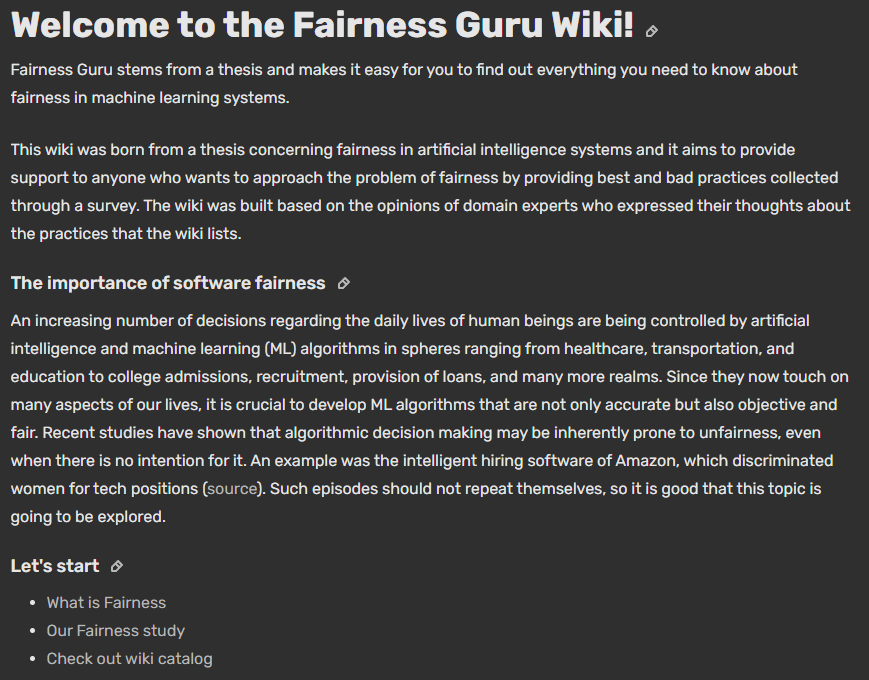
\includegraphics[width=400pt]{figure/catalog/welcome.png}
    \caption{Pagina principale della wiki}
    \label{wiki-welcome}
\end{figure}

Parlando del catalogo della wiki, sono riportate sia le cause delle discriminazioni che i pattern valutati durante la stesura del survey. Il catalogo (figura \ref{wiki-catalog}) suddivide le cause in due sezioni, cioè \emph{attributi sensibili} e \emph{aspetti legati al machine learning}; le practice sono suddivise, invece, in tre sezioni, cioè \emph{best practice}, \emph{bad practice}, \emph{practice non classificate}. Le practice sono state riportate nelle rispettive sezioni secondo quanto analizzato durante l'analisi dei dati.

\begin{figure}[h!]
    \centering
    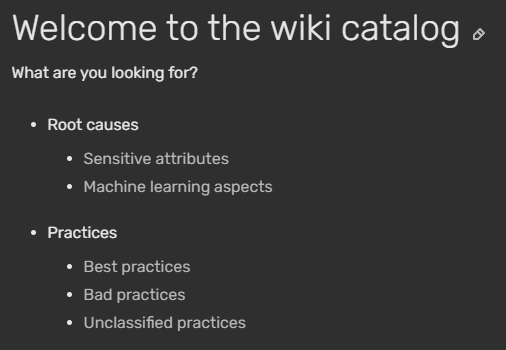
\includegraphics[width=300pt]{figure/catalog/catalog.png}
    \caption{Catalogo della wiki}
    \label{wiki-catalog}
\end{figure}

Le cause delle discriminazioni sono riportate fornendo al lettore i dati raccolti tramite il survey, mostrandoli sia in maniera grezza, in formato tabellare, sia tramite illustrazioni semplificate (figure \ref{im-a-root-1} e \ref{im-a-root-2}). Per gli attributi sensibili sono stati riportati anche le caratteristiche suggerite dai partecipanti (figure \ref{im-a-root-3} e \ref{wiki-suggestions}) in un'apposita domanda aperta di approfondimento, mentre per gli aspetti legati al machine learning sono state riportate definizioni utili a comprendere cosa sia ogni aspetto elencato. Ogni definizione è accompagnata dalla sorgente consultata per la stesura, utile nel caso il lettore voglia approfondire (figura \ref{wiki-links}).

\begin{figure}[h!]
    \centering
    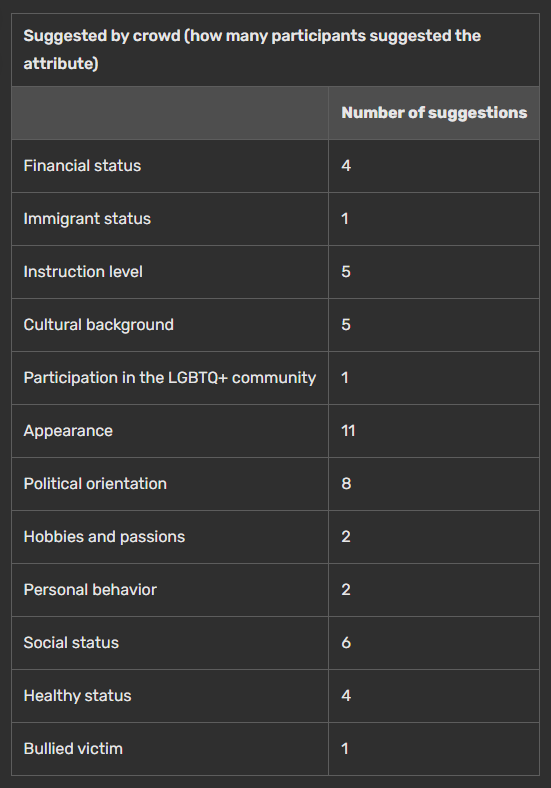
\includegraphics[width=300pt]{figure/catalog/suggests.png}
    \caption{Attributi sensibili suggeriti dai partecipanti, riportati nella wiki}
    \label{wiki-suggestions}
\end{figure}

\begin{figure}[h!]
    \centering
    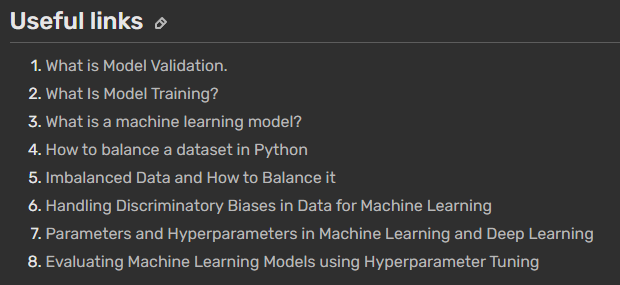
\includegraphics[width=360pt]{figure/catalog/links.png}
    \caption{Sorgenti di riferimento e di approfondimento della wiki}
    \label{wiki-links}
\end{figure}

Le practice, invece, sono state organizzate diversamente: per ogni classificazione è stata posta la lista di practice associate (figura \ref{wiki-prac-list}) e ognuna di esse viene illustrata in una apposita pagina dedicata. Ogni pagina dedicata alla classificazione delle practice contiene anche la definizione della classificazione e ricorda al lettore che i dati che verranno mostrati per ogni practice sono il risultato di un'analisi condotta sulle risposte di 120 partecipanti.\\

\begin{figure}[h!]
    \centering
    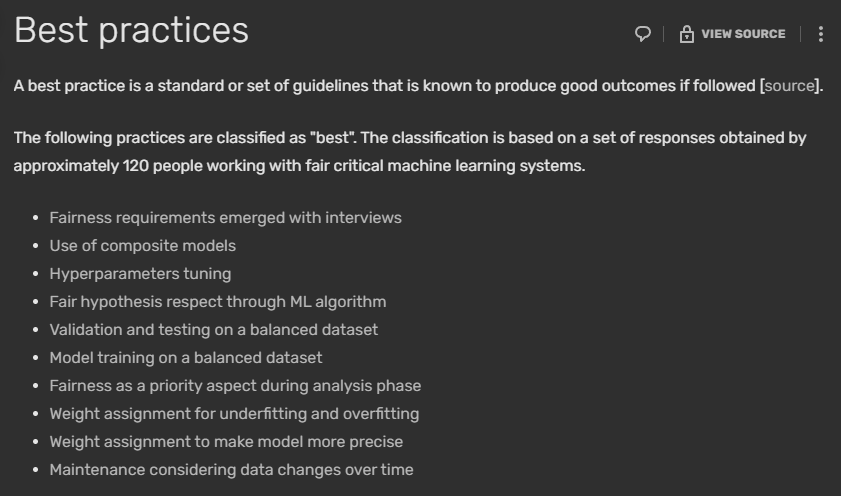
\includegraphics[width=420pt]{figure/catalog/best.png}
    \caption{Pagina della wiki dedicata alla categorizzazione}
    \label{wiki-prac-list}
\end{figure}

La pagina dedicata alla singola practice mostra tutti i dettagli utili a comprendere cosa tratti e se è considerata best o bad. Precisamente, il lettore viene introdotto alla pagina tramite una breve descrizione della practice, seguita immediatamente da una sezione che mostra, come per le cause di discriminazione, i dati dell'analisi tramite illustrazioni semplificate (figura \ref{wiki-analysis}). Segue, poi, una sezione inerente agli argomenti correlati alla practice: vengono trattate tutte le nozioni teoriche che riguardano strettamente la practice che il lettore sta visualizzando. Le nozioni teoriche riportate sono accompagnate dalle sorgenti da cui sono state ricavate (figura \ref{wiki-links}), ordinate in base all'ordine delle nozioni mostrate.

\begin{figure}[h!]
    \centering
    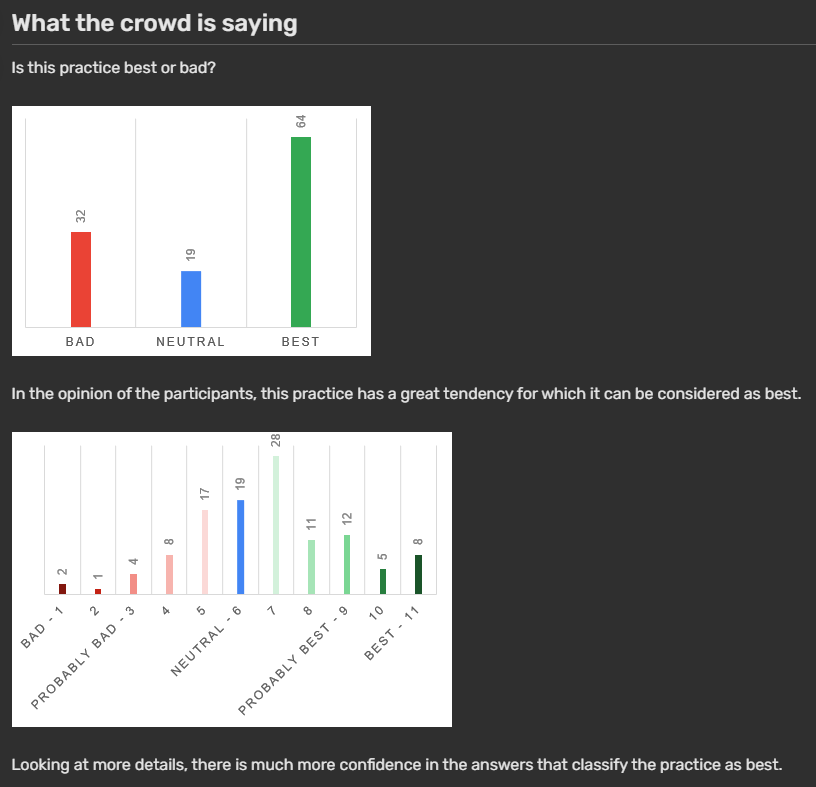
\includegraphics[width=420pt]{figure/catalog/crowd.png}
    \caption{Illustrazioni statistiche inerenti alla practice riportate sulla wiki}
    \label{wiki-analysis}
\end{figure}

\section{Validazione e raffinamento del catalogo}
La wiki risulta essere accessibile a tutti, ma modificabile solamente dall'amministratore: è stata intrapresa tale scelta per evitare che qualche malintenzionato distrugga il lavoro svolto. Allo stesso tempo, però, si vuole fare in modo che chiunque possa contribuire con informazioni valide e che la wiki rimanga sempre aggiornata secondo le indicazioni che partecipanti e lettori forniscono. Per invogliare a proporre modifiche, alla conclusione di ogni pagina inerente le cause di discriminazione e le practice è stata aggiunta una sezione (figura \ref{wiki-contribute}) in cui si spiega al visitatore come proporre modifiche: potrà farlo commentando la pagina, dato che ogni pagina è fornita di una sezione dedicata ai commenti, o inviando una email al sottoscritto. Ogni modifica proposta verrà accuratamente analizzata in modo da aggiungere sempre più contenuti e informazioni alla wiki.

\begin{figure}[h!]
    \centering
    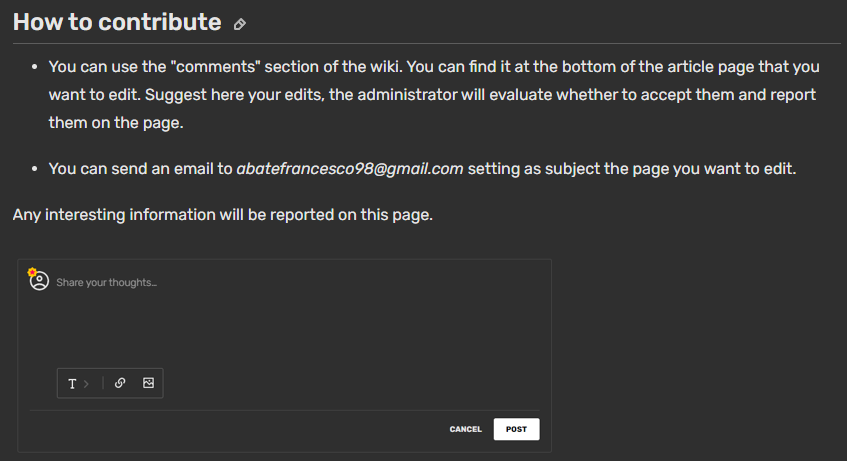
\includegraphics[width=420pt]{figure/catalog/contribute.png}
    \caption{Sezione inerente ai contributi da parte dei visitatori della wiki}
    \label{wiki-contribute}
\end{figure}

La wiki, a tal punto, può essere considerabile come soggetta ad un processo iterativo di raffinamento sulla base dei commenti ricevuti. Una prima iterazione consiste nel chiedere una revisione della wiki a tutti gli utenti che hanno dato il consenso per farsi contattare via email nella fase post esperimento; dopodiché, una volta analizzati i pareri ed eventualmente modificata la wiki, le successive iterazioni dipenderanno dai futuri visitatori. In generale, quindi, un'iterazione comprende l'analisi della proposta di modifica e, se accettata, l'applicazione dei cambiamenti. La proposta di modifica verrà accettata sulla base del giudizio personale dell'amministratore, il quale comprenderà se la modifica è sensata o meno. In caso di dubbi, sarà necessario sollevare un confronto con il visitatore che ha proposto la modifica, in modo da ottenere maggiori informazioni, comprendere la veridicità delle informazioni ove possibile e chiarire perché la sua proposta possa essere utile alla comunità.

\newpage